\documentclass[12pt,a4paper]{article}

% --------------------------------------------------
% Pacotes
% --------------------------------------------------
\usepackage[utf8]{inputenc}
\usepackage[T1]{fontenc}
\usepackage[brazilian]{babel}
\usepackage{amsmath}
\usepackage{amssymb}
\usepackage{graphicx}
\usepackage{float}
\usepackage{booktabs}
\usepackage{array}
\usepackage{geometry}
\usepackage{siunitx}
\usepackage{caption}
\usepackage{titlesec}
\usepackage{algorithm}
\usepackage{algpseudocode}

\geometry{
    left=2.5cm,
    right=2.5cm,
    top=2.5cm,
    bottom=2.5cm
}

\sisetup{
    output-decimal-marker = {,},
    per-mode = symbol
}

\setlength{\parindent}{1.25cm}
\setlength{\parskip}{0.1cm}

% Compactação vertical sem alterar o tamanho das figuras
\AtBeginDocument{
    \setlength{\abovedisplayskip}{4pt plus 1pt minus 1pt}
    \setlength{\belowdisplayskip}{4pt plus 1pt minus 1pt}
    \setlength{\abovedisplayshortskip}{2pt plus 1pt minus 1pt}
    \setlength{\belowdisplayshortskip}{2pt plus 1pt minus 1pt}
    \setlength{\jot}{2pt}
}

\titlespacing*{\section}{0pt}{8pt}{4pt}
\titlespacing*{\subsection}{0pt}{7pt}{3pt}
\titlespacing*{\subsubsection}{0pt}{5pt}{2pt}

\begin{document}

\begin{titlepage}
\begin{center}
% Logo da Instituição
\begin{figure}[H]
    \centering
    
\includegraphics[width=0.3\linewidth]{image.png}
\end{figure}
\vspace*{0.5cm}

% Cabeçalho
\textbf{\large UNIVERSIDADE FEDERAL DE MINAS GERAIS}\\
\textbf{\large ESCOLA DE ENGENHARIA}\\

\vspace{2.5cm}

% Integrantes e Matrículas
\large
Felipe Augusto Cruz Sousa -- 2019430481\\
Gustavo Madureira Tavares de Melo -- 2022055629\\
Henry Diniz Sepini Rodrigues Amaral -- 2022055653\\
Lucas Rodrigues Prosperi Ayala -- 2021019580\\
Luisa Marques Laboissiere -- 2022102856\\
Thales Gregory Vasconcelos Santos -- 2018019630\\

\vspace{3cm}

% Título do Trabalho
\textbf{\LARGE OTIMIZAÇÃO E DECISÃO MULTICRITÉRIO\\
\large Relatório final | Entrega 3}\\

\vspace{1.5cm}

% Informações da Disciplina
\textbf{\large Teoria da Decisão}\\

\vfill

% Local e Data
\textbf{\large Belo Horizonte}\\
\textbf{\large Novembro de 2026}
\end{center}
\end{titlepage}

\newpage
\tableofcontents
\newpage

% ============================================================
% FORMULAÇÃO DO PROBLEMA
% ============================================================

\section{Formulação do Problema}

\subsection{Descrição do problema}

O problema consiste na definição da composição de dez pilhas de minério
utilizadas para alimentar dois equipamentos de sinterização, denominados
Sinter 1 e Sinter 2. Cada equipamento é abastecido por um conjunto de cinco
pilhas, sendo que todas as pilhas associadas ao mesmo equipamento compartilham
os mesmos requisitos de qualidade.

Cada pilha deve atingir uma massa previamente especificada e é formada pela
combinação de diferentes minérios disponíveis no pátio da usina. Os minérios
possuem diferentes custos de aquisição e diferentes teores de ferro total
(FeT), sílica ($SiO_2$) e alumina ($Al_2O_3$).

O transporte dos minérios é realizado por caminhões com capacidade fixa de
$2$ kt. Portanto, a quantidade de minério destinada a cada pilha deve ser um
múltiplo da capacidade de um caminhão.

Além disso, existem restrições logísticas que determinam quais minérios podem
ser utilizados em cada equipamento de sinterização, bem como limites mínimos
e máximos de disponibilidade para cada minério.

O problema possui três objetivos, que nesta primeira etapa são considerados
separadamente:

\begin{enumerate}
    \item minimizar o custo total de aquisição dos minérios;
    \item minimizar a soma dos desvios quadráticos dos teores de $SiO_2$
    em relação ao valor-alvo de cada equipamento;
    \item minimizar a soma dos desvios quadráticos dos teores de $Al_2O_3$
    em relação ao valor-alvo de cada equipamento.
\end{enumerate}

Dessa forma, são considerados três problemas mono-objetivo com o mesmo
conjunto de variáveis e restrições, modificando-se apenas a função objetivo
otimizada em cada execução.


% ============================================================
% CONJUNTOS
% ============================================================

\subsection{Conjuntos e índices}

Sejam definidos os seguintes conjuntos:

\begin{itemize}
    \item $I = \{1,\ldots,n\}$: conjunto dos minérios disponíveis;
    \item $P = \{1,\ldots,10\}$: conjunto das pilhas;
    \item $G = \{1,2\}$: conjunto dos equipamentos de sinterização.
\end{itemize}

No conjunto de dados utilizado neste trabalho, existem vinte minérios,
portanto:

\begin{equation}
    I = \{1,\ldots,20\}.
\end{equation}

As pilhas são divididas entre os equipamentos da seguinte forma:

\begin{equation}
    P_1 = \{1,2,3,4,5\},
\end{equation}

\begin{equation}
    P_2 = \{6,7,8,9,10\}.
\end{equation}

Define-se ainda $g(p)$ como o equipamento de sinterização associado à
pilha $p$.


% ============================================================
% PARÂMETROS
% ============================================================

\subsection{Parâmetros}

Para cada minério $i \in I$, são considerados os seguintes parâmetros:

\begin{itemize}

    \item $c_i$: custo de aquisição do minério $i$, em R\$/t;

    \item $s_i$: teor de $SiO_2$ do minério $i$, em \%;

    \item $a_i$: teor de $Al_2O_3$ do minério $i$, em \%;

    \item $f_i$: teor de ferro total (FeT) do minério $i$, em \%;

    \item $D_i^{\min}$: disponibilidade mínima do minério $i$,
    em número de caminhões;

    \item $D_i^{\max}$: disponibilidade máxima do minério $i$,
    em número de caminhões.

\end{itemize}

Define-se ainda o parâmetro binário:

\begin{equation}
e_{ig} =
\begin{cases}
1, & \text{se o minério $i$ pode alimentar o equipamento $g$},\\
0, & \text{caso contrário}.
\end{cases}
\end{equation}

Para cada pilha $p \in P$, define-se:

\begin{equation}
    M_p = \text{massa final requerida para a pilha $p$, em kt}.
\end{equation}

A capacidade fixa de cada caminhão é dada por:

\begin{equation}
    C = 2 \text{ kt}.
\end{equation}

Como o custo dos minérios é expresso em R\$/t, também é utilizada a
capacidade em toneladas:

\begin{equation}
    C_t = 2000 \text{ t}.
\end{equation}

Para cada equipamento $g \in G$, são definidos os limites e valores-alvo
de qualidade:

\begin{itemize}

    \item $L_g^{Si}$: limite mínimo de $SiO_2$;

    \item $U_g^{Si}$: limite máximo de $SiO_2$;

    \item $T_g^{Si}$: valor-alvo de $SiO_2$;

    \item $L_g^{Al}$: limite mínimo de $Al_2O_3$;

    \item $U_g^{Al}$: limite máximo de $Al_2O_3$;

    \item $T_g^{Al}$: valor-alvo de $Al_2O_3$.

\end{itemize}


% ============================================================
% VARIÁVEL
% ============================================================

\subsection{Variável de decisão}

A variável de decisão é definida como:

\begin{equation}
    x_{ip} \in \mathbb{Z}_{\geq 0},
\end{equation}

onde $x_{ip}$ representa o número de caminhões do minério $i$ destinados
à pilha $p$.

Como cada caminhão possui capacidade de $2$ kt, a massa do minério $i$
utilizada na pilha $p$ é:

\begin{equation}
    2x_{ip} \text{ kt}.
\end{equation}


% ============================================================
% QUALIDADE DAS PILHAS
% ============================================================

\subsection{Cálculo da qualidade das pilhas}

O teor de $SiO_2$ resultante na pilha $p$ é calculado pela média ponderada
dos minérios utilizados:

\begin{equation}
Si_p =
\frac{
C\sum_{i\in I}s_i x_{ip}
}{
M_p
}.
\end{equation}

Como $C=2$ kt:

\begin{equation}
\boxed{
Si_p =
\frac{
2\sum_{i\in I}s_i x_{ip}
}{
M_p
}
}
\end{equation}

De forma análoga, o teor de $Al_2O_3$ é dado por:

\begin{equation}
\boxed{
Al_p =
\frac{
2\sum_{i\in I}a_i x_{ip}
}{
M_p
}
}
\end{equation}


% ============================================================
% RESTRIÇÕES
% ============================================================

\subsection{Restrições}

\subsubsection{Atendimento da massa das pilhas}

Cada pilha deve atingir exatamente sua massa especificada:

\begin{equation}
\boxed{
C\sum_{i\in I}x_{ip}=M_p,
\qquad
\forall p\in P
}
\end{equation}

ou, considerando $C=2$ kt:

\begin{equation}
\boxed{
2\sum_{i\in I}x_{ip}=M_p,
\qquad
\forall p\in P.
}
\end{equation}


\subsubsection{Limites de $SiO_2$}

O teor de $SiO_2$ de cada pilha deve estar dentro dos limites definidos
para o equipamento ao qual a pilha pertence:

\begin{equation}
\boxed{
L_{g(p)}^{Si}
\leq
\frac{
2\sum_{i\in I}s_i x_{ip}
}{
M_p
}
\leq
U_{g(p)}^{Si},
\qquad
\forall p\in P.
}
\end{equation}

Uma vez que $M_p$ é constante, essa restrição pode ser escrita como:

\begin{equation}
\boxed{
L_{g(p)}^{Si} M_p
\leq
2\sum_{i\in I}s_i x_{ip}
\leq
U_{g(p)}^{Si} M_p,
\qquad
\forall p\in P.
}
\end{equation}


\subsubsection{Limites de $Al_2O_3$}

Analogamente:

\begin{equation}
\boxed{
L_{g(p)}^{Al}
\leq
\frac{
2\sum_{i\in I}a_i x_{ip}
}{
M_p
}
\leq
U_{g(p)}^{Al},
\qquad
\forall p\in P.
}
\end{equation}

ou:

\begin{equation}
\boxed{
L_{g(p)}^{Al}M_p
\leq
2\sum_{i\in I}a_i x_{ip}
\leq
U_{g(p)}^{Al}M_p,
\qquad
\forall p\in P.
}
\end{equation}


\subsubsection{Compatibilidade entre minério e equipamento}

Cada minério pode ser utilizado apenas nos equipamentos para os quais
é considerado elegível. Dessa forma:

\begin{equation}
\boxed{
x_{ip}
\leq
D_i^{\max}e_{i,g(p)},
\qquad
\forall i\in I,\ \forall p\in P.
}
\end{equation}

Caso $e_{i,g(p)}=0$, tem-se necessariamente:

\begin{equation}
    x_{ip}=0.
\end{equation}


\subsubsection{Disponibilidade dos minérios}

A utilização total de cada minério deve respeitar seus limites mínimo
e máximo de disponibilidade:

\begin{equation}
\boxed{
D_i^{\min}
\leq
\sum_{p\in P}x_{ip}
\leq
D_i^{\max},
\qquad
\forall i\in I.
}
\end{equation}


\subsubsection{Integralidade}

Como cada unidade representa um caminhão completo:

\begin{equation}
\boxed{
x_{ip}\in\mathbb{Z}_{\geq0},
\qquad
\forall i\in I,\ \forall p\in P.
}
\end{equation}


% ============================================================
% OBJETIVOS
% ============================================================

\subsection{Funções objetivo}

\subsubsection{Minimização do custo total}

A primeira função objetivo considera o custo total de aquisição dos minérios.

Como $c_i$ é expresso em R\$/t e cada caminhão possui $2000$ toneladas,
a função objetivo é:

\begin{equation}
\boxed{
f_1(x)=
\sum_{p\in P}
\sum_{i\in I}
2000\,c_i x_{ip}
}
\end{equation}

O primeiro problema mono-objetivo é, portanto:

\begin{equation}
\boxed{
\min_{x\in X} f_1(x),
}
\end{equation}

onde $X$ representa o conjunto das soluções que satisfazem as restrições
do problema.


\subsubsection{Minimização do desvio de $SiO_2$}

Para cada pilha, calcula-se a diferença entre seu teor de $SiO_2$ e o
valor-alvo definido para o respectivo equipamento.

A segunda função objetivo é definida como:

\begin{equation}
\boxed{
f_2(x)=
\sum_{p\in P}
\left(
Si_p-T_{g(p)}^{Si}
\right)^2
}
\end{equation}

ou, substituindo $Si_p$:

\begin{equation}
\boxed{
f_2(x)=
\sum_{p\in P}
\left(
\frac{
2\sum_{i\in I}s_i x_{ip}
}{
M_p
}
-
T_{g(p)}^{Si}
\right)^2.
}
\end{equation}

O segundo problema mono-objetivo é:

\begin{equation}
\boxed{
\min_{x\in X} f_2(x).
}
\end{equation}


\subsubsection{Minimização do desvio de $Al_2O_3$}

De forma análoga, a terceira função objetivo é:

\begin{equation}
\boxed{
f_3(x)=
\sum_{p\in P}
\left(
Al_p-T_{g(p)}^{Al}
\right)^2
}
\end{equation}

ou:

\begin{equation}
\boxed{
f_3(x)=
\sum_{p\in P}
\left(
\frac{
2\sum_{i\in I}a_i x_{ip}
}{
M_p
}
-
T_{g(p)}^{Al}
\right)^2.
}
\end{equation}

O terceiro problema mono-objetivo é:

\begin{equation}
\boxed{
\min_{x\in X} f_3(x).
}
\end{equation}


% ============================================================
% CONJUNTO VIÁVEL
% ============================================================

\subsection{Síntese da formulação}

Os três problemas considerados nesta etapa compartilham o mesmo conjunto
viável:

\begin{equation}
X =
\left\{
x :
\begin{array}{l}
2\displaystyle\sum_{i\in I}x_{ip}=M_p,
\quad \forall p\in P,
\\[3mm]

L_{g(p)}^{Si}
\leq
\dfrac{
2\displaystyle\sum_{i\in I}s_i x_{ip}
}{
M_p
}
\leq
U_{g(p)}^{Si},
\quad \forall p\in P,
\\[4mm]

L_{g(p)}^{Al}
\leq
\dfrac{
2\displaystyle\sum_{i\in I}a_i x_{ip}
}{
M_p
}
\leq
U_{g(p)}^{Al},
\quad \forall p\in P,
\\[4mm]

D_i^{\min}
\leq
\displaystyle\sum_{p\in P}x_{ip}
\leq
D_i^{\max},
\quad \forall i\in I,
\\[3mm]

x_{ip}
\leq
D_i^{\max}e_{i,g(p)},
\quad \forall i\in I,\forall p\in P,
\\[3mm]

x_{ip}\in\mathbb{Z}_{\geq0}.
\end{array}
\right\}.
\end{equation}

Assim, os três problemas resolvidos nesta etapa são:

\begin{align}
P_1 &: \min_{x\in X} f_1(x),\\
P_2 &: \min_{x\in X} f_2(x),\\
P_3 &: \min_{x\in X} f_3(x).
\end{align}


% ============================================================
% OBSERVAÇÃO SOBRE FET
% ============================================================

\subsection{Tratamento do teor de ferro total}

Embora o teor de ferro total (FeT) esteja presente nos dados de entrada,
ele não é considerado como uma restrição ativa nesta etapa.

Os limites fornecidos para FeT são de $0\%$ e $100\%$, de forma que
qualquer combinação dos minérios disponíveis satisfaz automaticamente
esses valores. Consequentemente, o FeT não influencia a otimização
realizada neste estudo.


% ============================================================
% REPRESENTAÇÃO COMPUTACIONAL
% ============================================================

\section{Representação Computacional da Solução}

Para a implementação da metaheurística, optou-se por representar cada
pilha como um vetor de minérios, no qual cada posição corresponde a um
caminhão de $2$ kt.

Dessa forma, uma pilha de massa $M_p$ é representada por um vetor com:

\begin{equation}
n_p =
\frac{M_p}{2}
\end{equation}

posições.

Por exemplo, uma pilha com massa total de $20$ kt contém dez posições.
Uma possível representação é:

\begin{equation}
P_1 =
[M_4,M_4,M_{10},M_{10},M_{11},
M_{14},M_{14},M_{14},M_{14},M_{14}].
\end{equation}

Cada elemento do vetor identifica o minério transportado por um caminhão.
Essa representação foi escolhida por permitir que as estruturas de
vizinhança sejam implementadas diretamente por meio da alteração ou troca
das posições dos vetores.


% ============================================================
% SOLUÇÃO INICIAL
% ============================================================

\section{Heurística Construtiva da Solução Inicial}

A solução inicial é construída utilizando uma heurística gulosa baseada
no custo dos minérios.

O procedimento possui dois objetivos principais:

\begin{enumerate}

    \item garantir inicialmente o atendimento das restrições estruturais
    relacionadas à massa, compatibilidade e disponibilidade dos minérios;

    \item produzir rapidamente uma solução que possa ser posteriormente
    aprimorada pela metaheurística VNS/GVNS.

\end{enumerate}

Nesta etapa, não é exigido que a solução inicial respeite os limites de
qualidade de $SiO_2$ e $Al_2O_3$. Caso ocorram violações, estas serão
tratadas posteriormente pela estratégia de busca.


\subsection{Etapas da construção}

A heurística é dividida em duas etapas.

\subsubsection{Atendimento das disponibilidades mínimas}

Inicialmente, são identificados todos os minérios que possuem
disponibilidade mínima obrigatória.

Para cada minério $i$, são adicionados $D_i^{\min}$ caminhões às pilhas,
respeitando:

\begin{itemize}

    \item a compatibilidade do minério com o equipamento;

    \item a capacidade máxima da pilha.

\end{itemize}

A utilização de cada minério é atualizada após cada inserção.


\subsubsection{Preenchimento das pilhas}

Após o atendimento das disponibilidades mínimas, as pilhas são percorridas
sequencialmente.

Para cada pilha, são identificados os minérios compatíveis com o
equipamento correspondente e esses minérios são ordenados em ordem
crescente de custo.

Enquanto houver posições disponíveis na pilha, seleciona-se o minério
compatível de menor custo que ainda possua disponibilidade.

O procedimento é repetido até que todas as pilhas atinjam suas respectivas
massas.


% ============================================================
% PSEUDOCÓDIGO
% ============================================================

\subsection{Pseudocódigo da heurística construtiva}

O Algoritmo~\ref{alg:construtiva} apresenta o procedimento utilizado
para construir a solução inicial.

\begin{algorithm}[H]

\caption{Heurística construtiva da solução inicial}
\label{alg:construtiva}

\begin{algorithmic}[1]

\State Criar todas as pilhas inicialmente vazias
\State Inicializar $uso_i \gets 0$, $\forall i\in I$

\For{cada minério $i\in I$}

    \For{$k=1$ até $D_i^{\min}$}

        \State Encontrar uma pilha $p$ com espaço disponível
        \Statex \hspace{\algorithmicindent}
        e tal que $e_{i,g(p)}=1$

        \State Inserir o minério $i$ na pilha $p$

        \State $uso_i \gets uso_i + 1$

    \EndFor

\EndFor

\For{cada pilha $p\in P$}

    \State Construir o conjunto de minérios elegíveis para $g(p)$

    \State Ordenar os minérios elegíveis por custo crescente

    \While{$|P_p| < M_p/2$}

        \State Selecionar o minério elegível $i$ de menor custo

        \Statex \hspace{\algorithmicindent}
        tal que $uso_i < D_i^{\max}$

        \State Inserir $i$ na pilha $p$

        \State $uso_i \gets uso_i + 1$

    \EndWhile

\EndFor

\State \Return solução construída

\end{algorithmic}

\end{algorithm}


% ============================================================
% VIABILIDADE
% ============================================================

\section{Avaliação da Solução Inicial}

Para facilitar o tratamento das soluções durante a metaheurística,
a viabilidade foi dividida em duas categorias: viabilidade estrutural
e viabilidade de qualidade.


\subsection{Viabilidade estrutural}

Uma solução é considerada estruturalmente viável quando satisfaz
simultaneamente:

\begin{enumerate}

    \item a massa exata de cada pilha;

    \item a compatibilidade entre minério e equipamento;

    \item a disponibilidade mínima de cada minério;

    \item a disponibilidade máxima de cada minério.

\end{enumerate}

A heurística construtiva foi desenvolvida de forma a preservar essas
restrições durante a construção da solução.


\subsection{Viabilidade de qualidade}

Separadamente, verifica-se se cada pilha satisfaz os limites de $SiO_2$
e $Al_2O_3$ definidos para seu respectivo equipamento.

Para $SiO_2$, verifica-se:

\begin{equation}
L_{g(p)}^{Si}
\leq
Si_p
\leq
U_{g(p)}^{Si}.
\end{equation}

Para $Al_2O_3$:

\begin{equation}
L_{g(p)}^{Al}
\leq
Al_p
\leq
U_{g(p)}^{Al}.
\end{equation}

A solução inicial pode apresentar violações dessas restrições. Essa
possibilidade é prevista no procedimento proposto, uma vez que a
heurística construtiva prioriza inicialmente a obtenção de uma solução
estruturalmente consistente.

O tratamento das violações de qualidade é incorporado à estratégia
de busca da metaheurística VNS/GVNS.


% ============================================================
% AVALIAÇÃO DOS OBJETIVOS
% ============================================================

\section{Avaliação das Funções Objetivo}

Após a construção da solução inicial, são calculados os três valores de
função objetivo:

\begin{equation}
f_1(x),
\qquad
f_2(x),
\qquad
f_3(x).
\end{equation}

O primeiro representa o custo total da composição, enquanto os demais
representam a dispersão dos valores de $SiO_2$ e $Al_2O_3$ em relação
aos respectivos alvos.

Esses valores são utilizados como referência inicial para a etapa de
busca. Em cada execução mono-objetivo, a VNS/GVNS utiliza uma das
funções $f_1$, $f_2$ ou $f_3$ como critério principal para avaliar
a melhoria das soluções candidatas.


% ============================================================
% METAHEURÍSTICA GVNS
% ============================================================

\section{Metaheurística GVNS}

A metaheurística adotada é a \textit{General Variable Neighborhood
Search} (GVNS), combinando a perturbação SHAKE do VNS com um refinamento
interno por \textit{Variable Neighborhood Descent} (VND).


\subsection{Tratamento de inviabilidade}

A estratégia adotada distingue dois tipos de inviabilidade, cada um tratado de
maneira diferente.

\textbf{Restrições estruturais} (massa das pilhas, compatibilidade entre minério e
equipamento, disponibilidade mínima e máxima de cada minério): qualquer movimento
que as viole é \emph{rejeitado}. Essa escolha decorre da natureza física dessas restrições:
a massa de cada pilha é determinada logisticamente pelo número de caminhões alocados, a
elegibilidade de minérios é um critério operacional fixo do processo de sinterização e os
limites de disponibilidade refletem contratos de fornecimento. Preservar essas restrições
por construção simplifica a avaliação de cada candidato e elimina a necessidade de reparo
posterior.

\textbf{Restrições de qualidade} ($SiO_2$ e $Al_2O_3$ fora dos limites): tratadas por
\emph{penalização}, permitindo que a busca explore temporariamente regiões de inviabilidade
de qualidade. Isso é desejável porque certas melhorias exigem atravessar composições
intermediárias que violam momentaneamente os limites, em particular quando múltiplas pilhas
precisam ser ajustadas em conjunto. A função de \textit{fitness} utilizada é:
\begin{equation}
    \phi(x) = f(x) + \lambda \cdot \text{pen}(x),
\end{equation}
onde
\begin{equation}
\begin{aligned}
    \text{pen}(x) = \sum_{p \in P} \bigl[{}
        &\max\!\left(0,\, L_{g(p)}^{Si} - Si_p\right)^2
       + \max\!\left(0,\, Si_p - U_{g(p)}^{Si}\right)^2 \\
        &+ \max\!\left(0,\, L_{g(p)}^{Al} - Al_p\right)^2
       + \max\!\left(0,\, Al_p - U_{g(p)}^{Al}\right)^2
    \bigr].
\end{aligned}
\end{equation}

Os pesos de penalidade foram definidos levando em conta a escala de cada função objetivo:
\begin{equation}
    \lambda_{f_1} = 10^{12}, \qquad
    \lambda_{f_2} = \lambda_{f_3} = 10^{4}.
\end{equation}

Os pesos preservam a configuração histórica do TP1 e desencorajam violações
na escala de cada objetivo. Contudo, uma penalidade finita não equivale a
normalização, não substitui a verificação das restrições e não garante que a
trajetória termine em uma solução viável.

Por isso, a implementação corrigida mantém dois registros independentes:
a incumbente da trajetória, comparada por $\phi$, e a melhor solução
fisicamente viável observada, comparada pelo objetivo bruto $f$.
Todo candidato estruturalmente válido avaliado no SHAKE, no VND ou no laço
externo é observado antes da decisão de aceitação. Uma solução viável pode
ser preservada mesmo que não substitua a incumbente por fitness. O retorno
usa uma cópia da melhor viável, quando encontrada. Caso contrário, a execução
é registrada como sem solução viável encontrada, sem certificar inviabilidade
matemática e sem inserir um valor fictício nas estatísticas.

\subsection{Estruturas de vizinhança}

Foram definidas três estruturas de vizinhança, aplicadas tanto no SHAKE
quanto no VND:

\begin{itemize}
    \item $N_1$: substitui \emph{um} caminhão numa pilha por outro
    minério compatível com o equipamento correspondente. A implementação enumera os movimentos compatíveis e sorteia uniformemente
    um deles. A distribuição é uniforme entre movimentos, não necessariamente
    entre pilhas.

    \item $N_2$: troca um caminhão entre duas pilhas \emph{distintas}.
    Dadas as pilhas $p_1$ e $p_2$, sorteia-se aleatoriamente uma posição
    em cada uma. O movimento é executado somente quando há
    \emph{compatibilidade cruzada}: o minério retirado de $p_1$ deve ser
    elegível para o equipamento de $p_2$, e o minério retirado de $p_2$
    deve ser elegível para o equipamento de $p_1$. Movimentos que não
    atendam a essa condição são descartados. Quando válido, o movimento
    preserva a massa de ambas as pilhas e a contagem global de cada minério.

    \item $N_3$: substitui \emph{dois} caminhões na \emph{mesma} pilha
    simultaneamente. Sorteia-se uma pilha, duas posições distintas e dois
    novos minérios compatíveis. O movimento exige que ambas as posições
    sejam efetivamente alteradas e que a composição resultante difira da
    original (não é mera permutação interna).

    A escolha dessa vizinhança se justifica pelos seguintes motivos:
    \begin{itemize}
        \item $N_1$ altera apenas uma posição por vez. Certas melhorias de
        qualidade --- como reduzir o teor de $SiO_2$ e ao mesmo tempo
        aumentar o de $Al_2O_3$ --- podem não ser alcançáveis com uma
        única substituição sem piorar o \textit{fitness} no passo
        intermediário. $N_3$ permite realizar esse tipo de ajuste combinado
        em uma única etapa.
        \item $N_2$ promove a redistribuição de minérios \emph{entre} pilhas,
        preservando a massa das pilhas envolvidas e a quantidade global
        utilizada de cada minério. Já $N_3$ altera diretamente a composição
        de uma \emph{única} pilha por meio de duas substituições simultâneas,
        possuindo lógica de movimento distinta das duas vizinhanças
        anteriores, conforme exigido pelo enunciado.
        \item Movimentos de maior amplitude permitem explorar regiões do
        espaço de busca que $N_1$ isolado alcançaria apenas após múltiplos
        passos, reduzindo o risco de estagnação em ótimos locais rasos.
    \end{itemize}
\end{itemize}

Por razões de desempenho computacional, $N_2$ e $N_3$ são implementadas
por amostragem aleatória em vez de enumeração exaustiva ($N_2$: 40
tentativas; $N_3$: 50 tentativas por pilha).


\subsection{Perturbação (SHAKE)}

O SHAKE aplica $k$ movimentos aleatórios extraídos das três vizinhanças,
com $k$ variando de $1$ a $K_{\max} = 3$. Cada movimento é aceito apenas
se a solução resultante for estruturalmente viável.


\subsection{VND — Variable Neighborhood Descent}

O VND percorre as vizinhanças $N_1 \to N_2 \to N_3$ em sequência.
Em cada vizinhança aplica-se busca local com \textit{First Improvement}
por amostragem ($\text{MAX\_AMOSTRAS} = 20$ vizinhos por chamada).
Ao encontrar melhoria, a solução é atualizada e o algoritmo retorna à $N_1$
(reinício clássico do VND), desde que o limite de reinícios não tenha sido
atingido ($\text{MAX\_RESTARTS\_VND} = 5$). Após atingir esse limite, o
algoritmo mantém a vizinhança atual enquanto encontra melhoria. O avanço
para a próxima ocorre somente quando não há melhoria; por exemplo, uma
melhoria em $N_2$ mantém a busca em $N_2$. O limite de reinícios não é
um teto do número de avaliações.


\subsection{Critério de Aceitação}

Em todas as etapas do algoritmo, o critério de aceitação é baseado em
melhoria estrita da função \textit{fitness}:

\begin{itemize}
    \item \textbf{VND --- busca local}: um vizinho $x'$ substitui a
    solução atual quando $\phi(x') < \phi(x_{\text{atual}})$. Empates
    não são aceitos. Ao encontrar o primeiro vizinho com \textit{fitness}
    menor (\textit{First Improvement}), a solução é atualizada imediatamente
    sem examinar os demais vizinhos da amostra.

    \item \textbf{Laço externo do GVNS}: a solução pós-VND $x''$ substitui
    a incumbente $x^*$ quando $\phi(x'') < \phi^*$. Após uma melhoria,
    $k$ é reiniciado para $1$ (retorno à perturbação mais fraca). Se $x''$
    não melhora $x^*$ para nenhum $k \leq K_{\max}$, a iteração externa
    encerra sem atualizar a incumbente.
\end{itemize}


\subsection{Laço externo do GVNS}

O Algoritmo~\ref{alg:gvns} apresenta o pseudocódigo do laço principal.

\begin{algorithm}[H]
\caption{GVNS mono-objetivo}
\label{alg:gvns}
\begin{algorithmic}[1]
\State $x \gets \text{SolucaoInicial}()$
\State $x^* \gets x$;\ $\phi^* \gets \phi(x^*)$;\ $x_v \gets \varnothing$
\State observar $x$ e atualizar $x_v$ se fisicamente viável
\State $\textit{sem\_melhora} \gets 0$
\For{$\textit{iter} = 1$ \textbf{to} $\text{MAX\_ITER}$}
    \State $k \gets 1$
    \While{$k \leq K_{\max}$}
        \State $x' \gets \text{SHAKE}(x^*,\, k)$
        \State $x'' \gets \text{VND}(x',\, f)$
        \State atualizar $x_v$ com cada candidato avaliado no SHAKE/VND
        \If{$\phi(x'') < \phi^*$}
            \State $x^* \gets x''$;\ $\phi^* \gets \phi(x'')$;\ $k \gets 1$
        \Else
            \State $k \gets k + 1$
        \EndIf
    \EndWhile
    \If{houve melhora nesta iteração}
        \State $\textit{sem\_melhora} \gets 0$
    \Else
        \State $\textit{sem\_melhora} \gets \textit{sem\_melhora} + 1$
        \If{$\textit{sem\_melhora} \geq \text{MAX\_SEM\_MELHORA}$}
            \State \textbf{break}
        \EndIf
    \EndIf
\EndFor
\If{$x_v \neq \varnothing$}
    \State \Return $x_v$ \Comment{Melhor viável observada por objetivo bruto}
\Else
    \State \Return status sem solução viável encontrada
\EndIf
\end{algorithmic}
\end{algorithm}

Os parâmetros do algoritmo estão resumidos na Tabela~\ref{tab:parametros}.

\begin{table}[H]
\centering
\caption{Parâmetros do GVNS}
\label{tab:parametros}
\small
\begin{tabular}{@{}l r p{0.52\textwidth}@{}}
\toprule
Parâmetro & Valor & Descrição \\
\midrule
$\text{MAX\_ITER}$         & 200 & Iterações externas por execução (critério de parada) \\
$K_{\max}$                 & 3   & Intensidades de perturbação no SHAKE \\
$\text{MAX\_AMOSTRAS}$     & 20  & Vizinhos amostrados por chamada de busca local (VND) \\
$\text{MAX\_RESTARTS\_VND}$& 5   & Reinícios internos máximos do VND \\
$\text{MAX\_SEM\_MELHORA}$ & 60  & Iterações sem melhora para parada antecipada \\
\bottomrule
\end{tabular}
\end{table}


\subsection{Critérios de Parada}

O algoritmo possui dois critérios de parada, aplicados por execução:

\begin{enumerate}
    \item \textbf{Número máximo de iterações} ($\text{MAX\_ITER} = 200$):
    interrompe a execução após 200 iterações externas do GVNS,
    independentemente de ter havido melhora recente.

    \item \textbf{Parada antecipada por estagnação}
    ($\text{MAX\_SEM\_MELHORA} = 60$): se $\phi^*$ não melhora por 60
    iterações externas consecutivas, a execução é interrompida antes de
    atingir $\text{MAX\_ITER}$. A revisão registra o motivo de término,
    as avaliações, as iterações e o tempo decorrido de cada execução.
\end{enumerate}

Os demais parâmetros da Tabela~\ref{tab:parametros} controlam a extensão
de cada etapa interna, sem constituir critérios de parada:
$K_{\max}$ define o número de intensidades de perturbação disponíveis;
$\text{MAX\_AMOSTRAS}$ controla o número de vizinhos amostrados por chamada;
e $\text{MAX\_RESTARTS\_VND}$ limita apenas os retornos à primeira vizinhança.
A API permite um teto opcional de avaliações, não utilizado nesta campanha TP1.
Os valores adotados foram definidos como configuração de referência para
os experimentos desta entrega; uma análise de sensibilidade paramétrica
constitui extensão natural deste trabalho.


% ============================================================
% RESULTADOS
% ============================================================


% Conteúdo de results/tp1_corrigido/resultados_tp1.tex
\section{Resultados Computacionais}

\subsection{Planejamento e validação dos experimentos}

Esta revisão reexecutou os três problemas em cinco sementes ($42$, $123$, $456$, $789$, $1011$), totalizando 15 buscas. Os parâmetros da Tabela~\ref{tab:parametros} e os pesos históricos de penalidade foram preservados. O retorno passou a ser a melhor solução viável observada, independentemente da incumbente por fitness.

Cada rodada tem composição, três objetivos, violações, status, histórico, contadores, motivo de parada e tempo decorrido em JSON. A releitura recalcula os valores; uma segunda rotina confere massa, compatibilidade, usos globais, faixas químicas e objetivos por contagens de minérios. As 15 soluções finais passaram pelas duas verificações. As estatísticas usam desvio-padrão amostral com denominador $n-1$.

\begin{table}[H]\centering\small

\caption{Resultados finais viáveis das cinco execuções por objetivo. Cada coluna corresponde a um problema otimizado separadamente.}

\label{tab:resultados}

\begin{tabular}{lrrr}\toprule

Execução & $f_1$ (R\$) & $f_2$ (p.p.$^2$) & $f_3$ (p.p.$^2$) \\ \midrule

1 (seed 42) & \num{60680000} & \num{2.373029} & \num{1.453254} \\

2 (seed 123) & \num{60400000} & \num{2.373828} & \num{1.450865} \\

3 (seed 456) & \num{60660000} & \num{2.372757} & \num{1.452078} \\

4 (seed 789) & \num{60300000} & \num{2.373927} & \num{1.436169} \\

5 (seed 1011) & \num{60480000} & \num{2.373844} & \num{1.443334} \\

\midrule

Mínimo & \num{60300000} & \num{2.372757} & \num{1.436169} \\

Média & \num{60504000} & \num{2.373477} & \num{1.447140} \\

Desvio-padrão & \num{164560} & \num{0.000543} & \num{0.007254} \\

Máximo & \num{60680000} & \num{2.373927} & \num{1.453254} \\

\bottomrule\end{tabular}\end{table}

\subsection{Esforço e parada}

Os tempos abaixo são de relógio e dependem da máquina e da instrumentação. Não são tempos de CPU nem devem ser comparados diretamente aos do log antigo.

\begin{table}[H]\centering\small

\caption{Esforço da campanha corrigida por objetivo}

\begin{tabular}{lrrrr}\toprule

Objetivo & Tempo médio (s) & Avaliações médias & Máx. iterações & Estagnação \\ \midrule

$f_1$ & \num{47.9} & \num{49434} & 4 & 1 \\

$f_2$ & \num{60.5} & \num{53562} & 2 & 3 \\

$f_3$ & \num{74.0} & \num{69886} & 5 & 0 \\

\bottomrule\end{tabular}\end{table}

\subsection{Curvas de convergência}

Cada figura sobrepõe as cinco sementes. O eixo vertical representa a melhor solução viável já observada, não o objetivo bruto da trajetória penalizada. Antes do primeiro candidato viável o valor é ausente; após esse momento, a curva não aumenta. A construtiva ($f_1=60{.}400{.}000$ R\$, $f_2\approx23{,}481055$, $f_3\approx14{,}909888$) tem 12 violações químicas e é apenas ponto de partida.

\begin{figure}[H]\centering

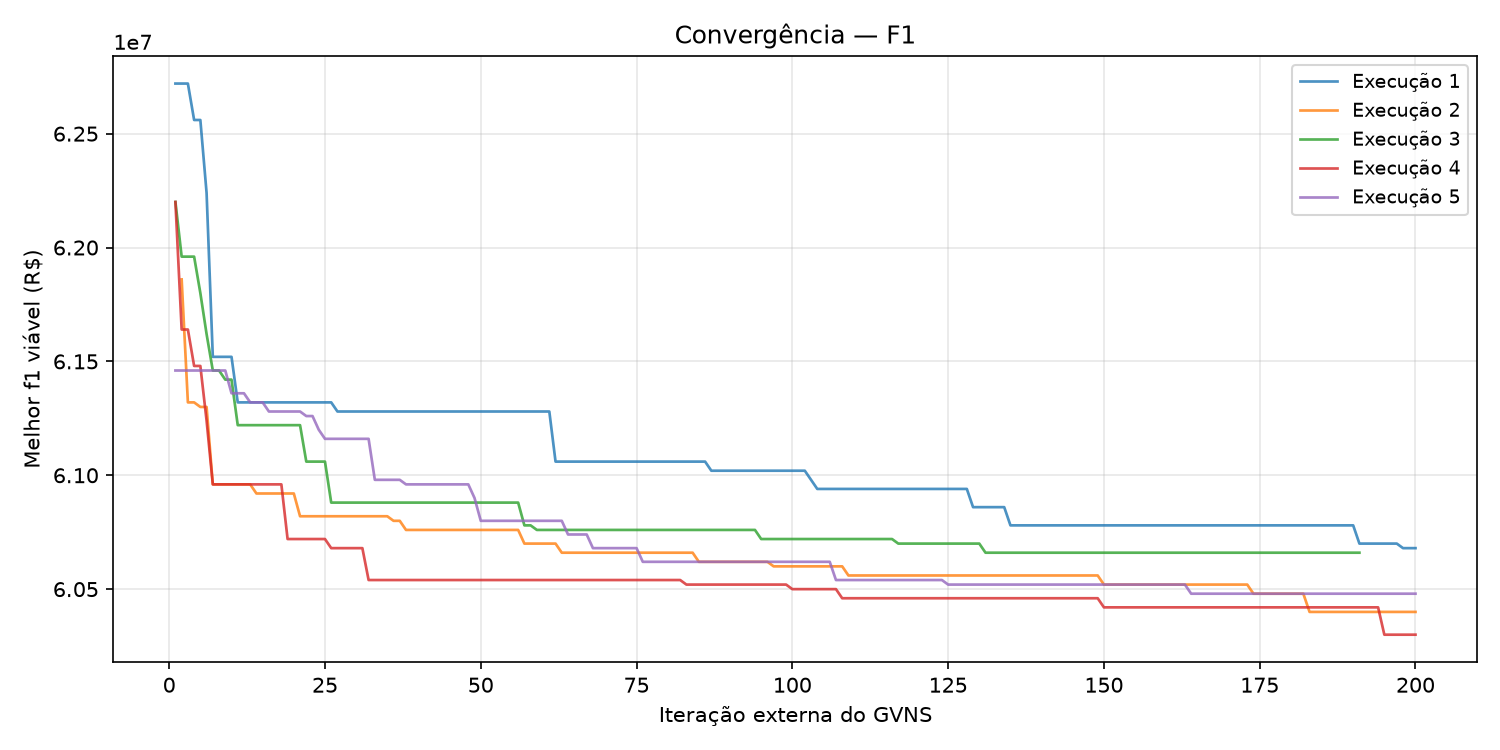
\includegraphics[width=0.88\textwidth]{results/tp1_corrigido/convergencia_f1.png}

\caption{Melhor valor viável observado de $f_1$ nas cinco execuções}

\label{fig:conv_f1}

\end{figure}

\begin{figure}[H]\centering

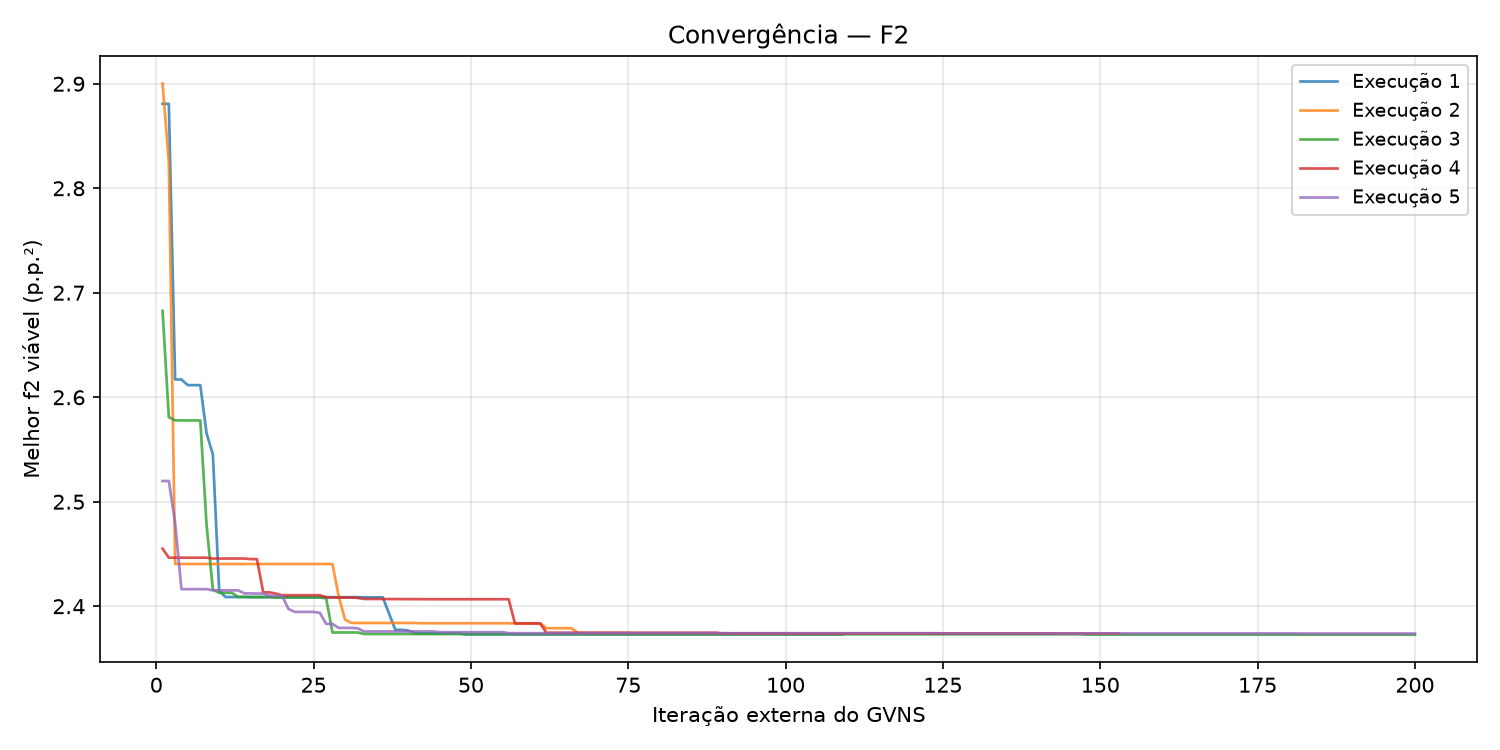
\includegraphics[width=0.88\textwidth]{results/tp1_corrigido/convergencia_f2.png}

\caption{Melhor valor viável observado de $f_2$ nas cinco execuções}

\label{fig:conv_f2}

\end{figure}

\begin{figure}[H]\centering

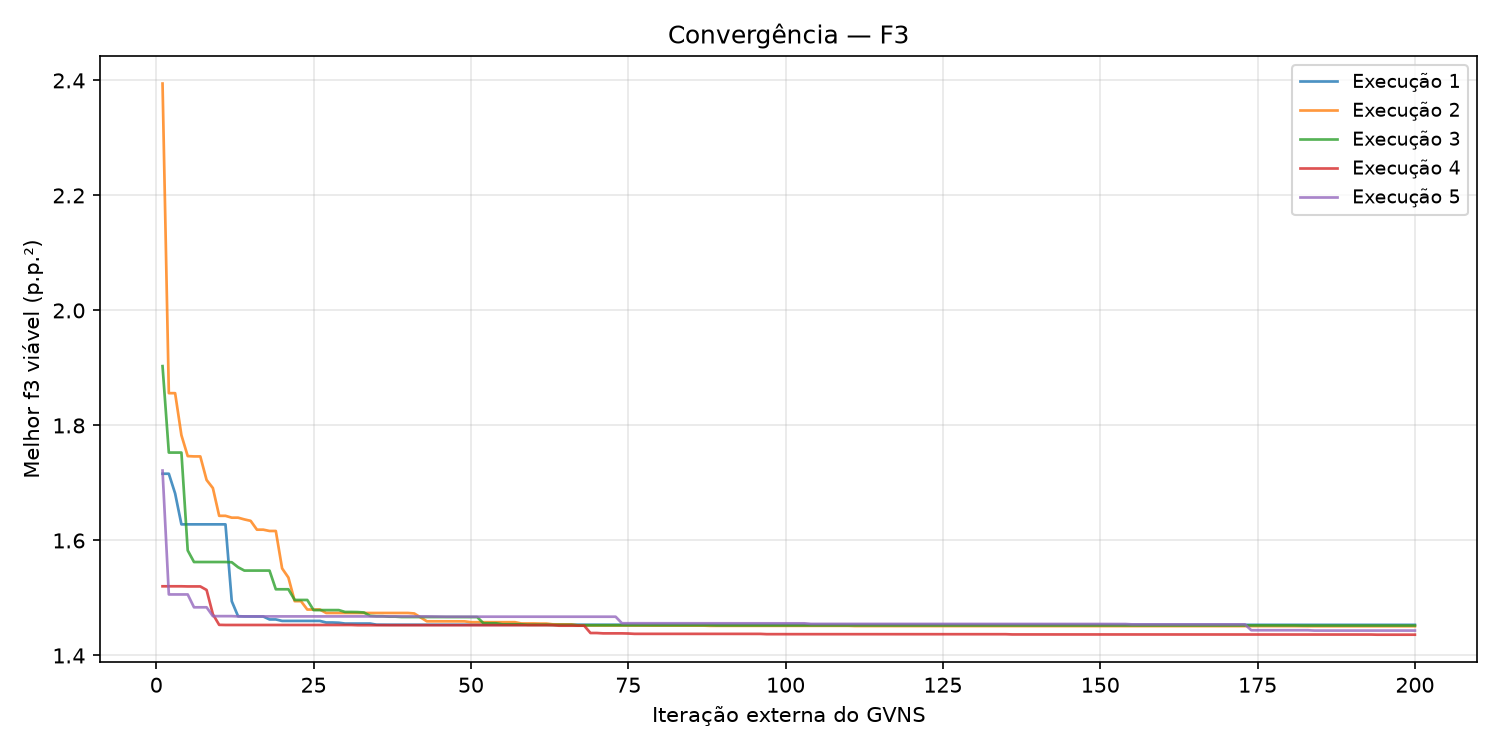
\includegraphics[width=0.88\textwidth]{results/tp1_corrigido/convergencia_f3.png}

\caption{Melhor valor viável observado de $f_3$ nas cinco execuções}

\label{fig:conv_f3}

\end{figure}

\subsection{Melhores composições e compromissos}

As barras mostram caminhões de 2 kt por minério em cada pilha; as alturas vão de 10 a 19 caminhões. As composições completas estão nos registros JSON.

\begin{figure}[H]\centering

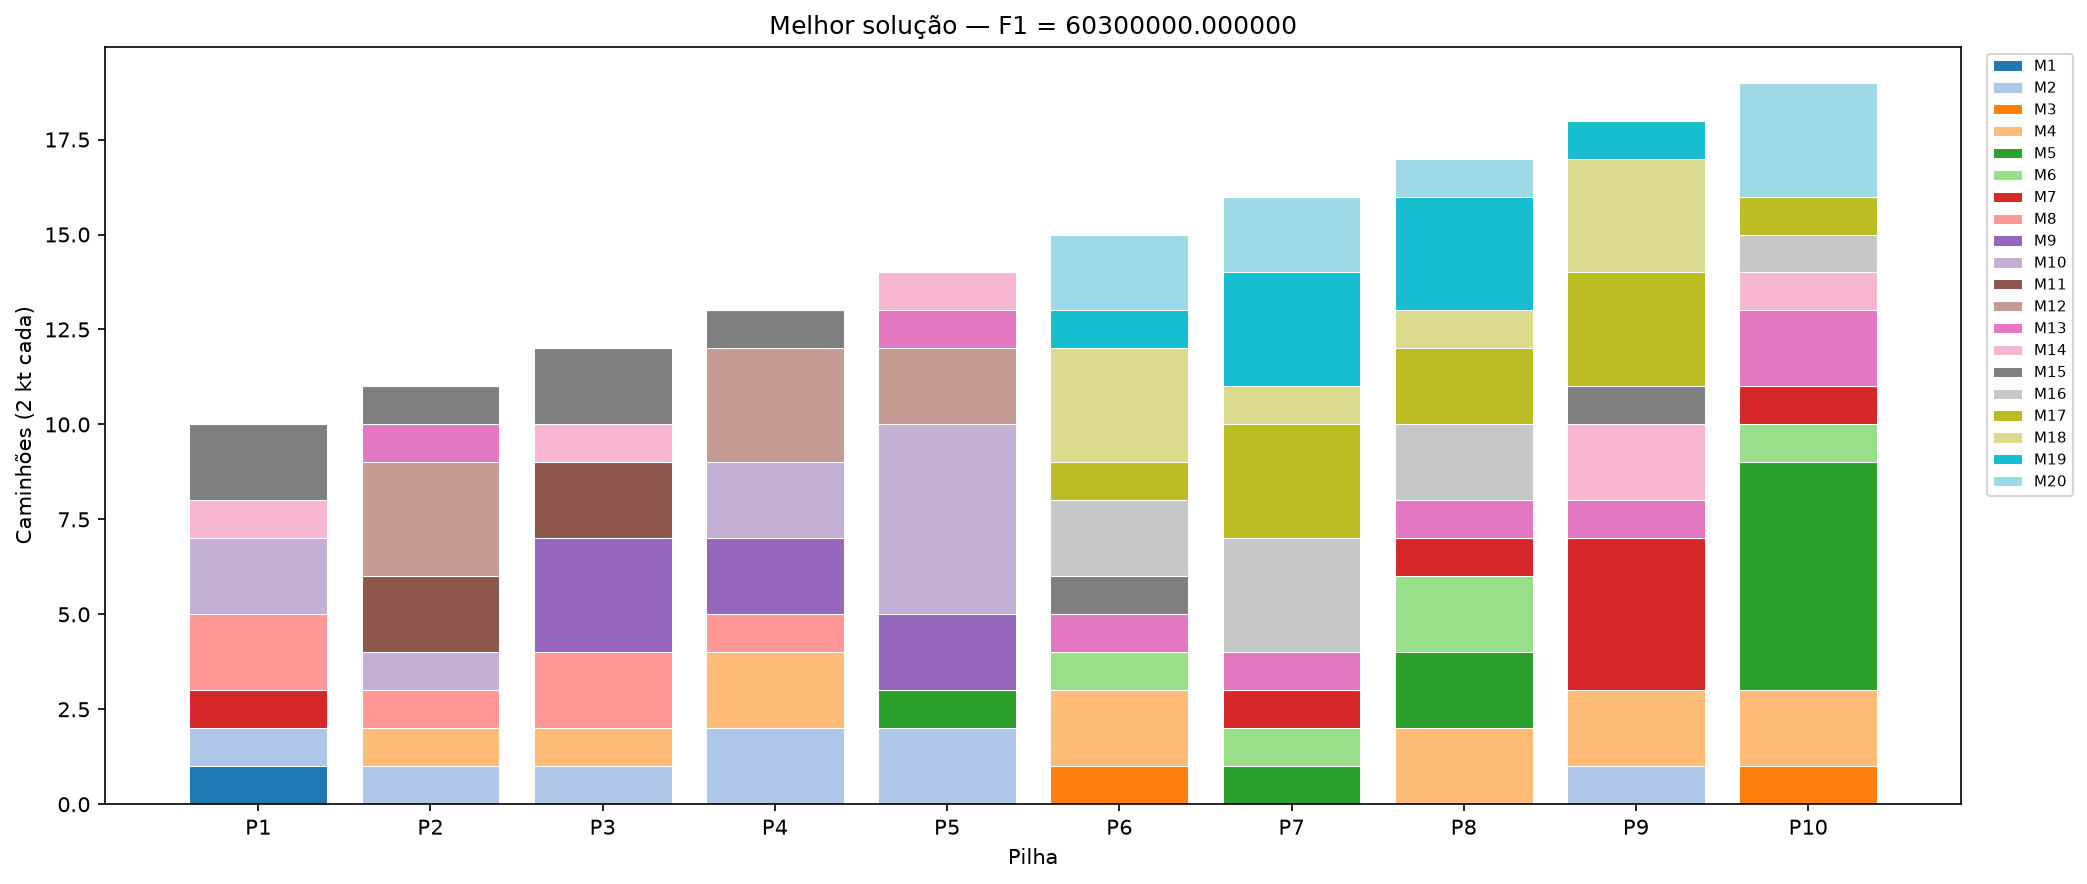
\includegraphics[width=\textwidth]{results/tp1_corrigido/melhor_solucao_f1.png}

\caption{Melhor composição para $f_1=\num{60300000}$ (seed 789)}

\label{fig:sol_f1}

\end{figure}

\begin{figure}[H]\centering

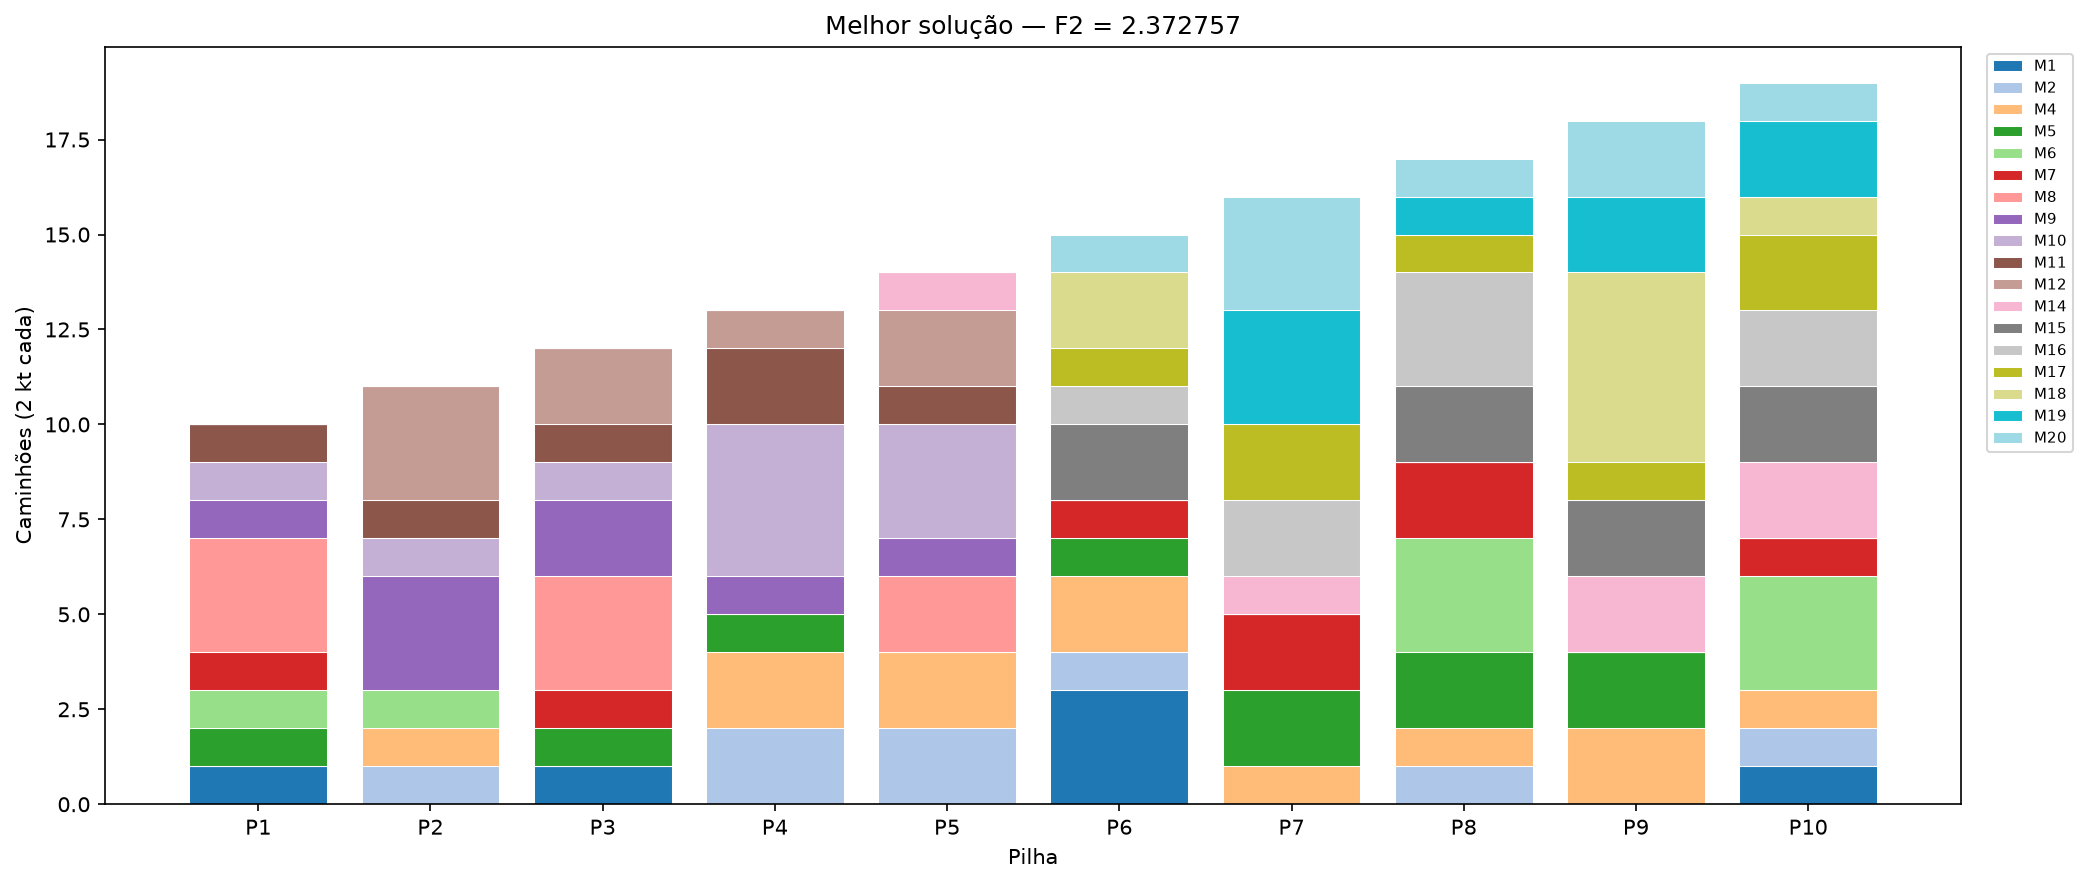
\includegraphics[width=\textwidth]{results/tp1_corrigido/melhor_solucao_f2.png}

\caption{Melhor composição para $f_2=\num{2.372757}$ (seed 456)}

\label{fig:sol_f2}

\end{figure}

\begin{figure}[H]\centering

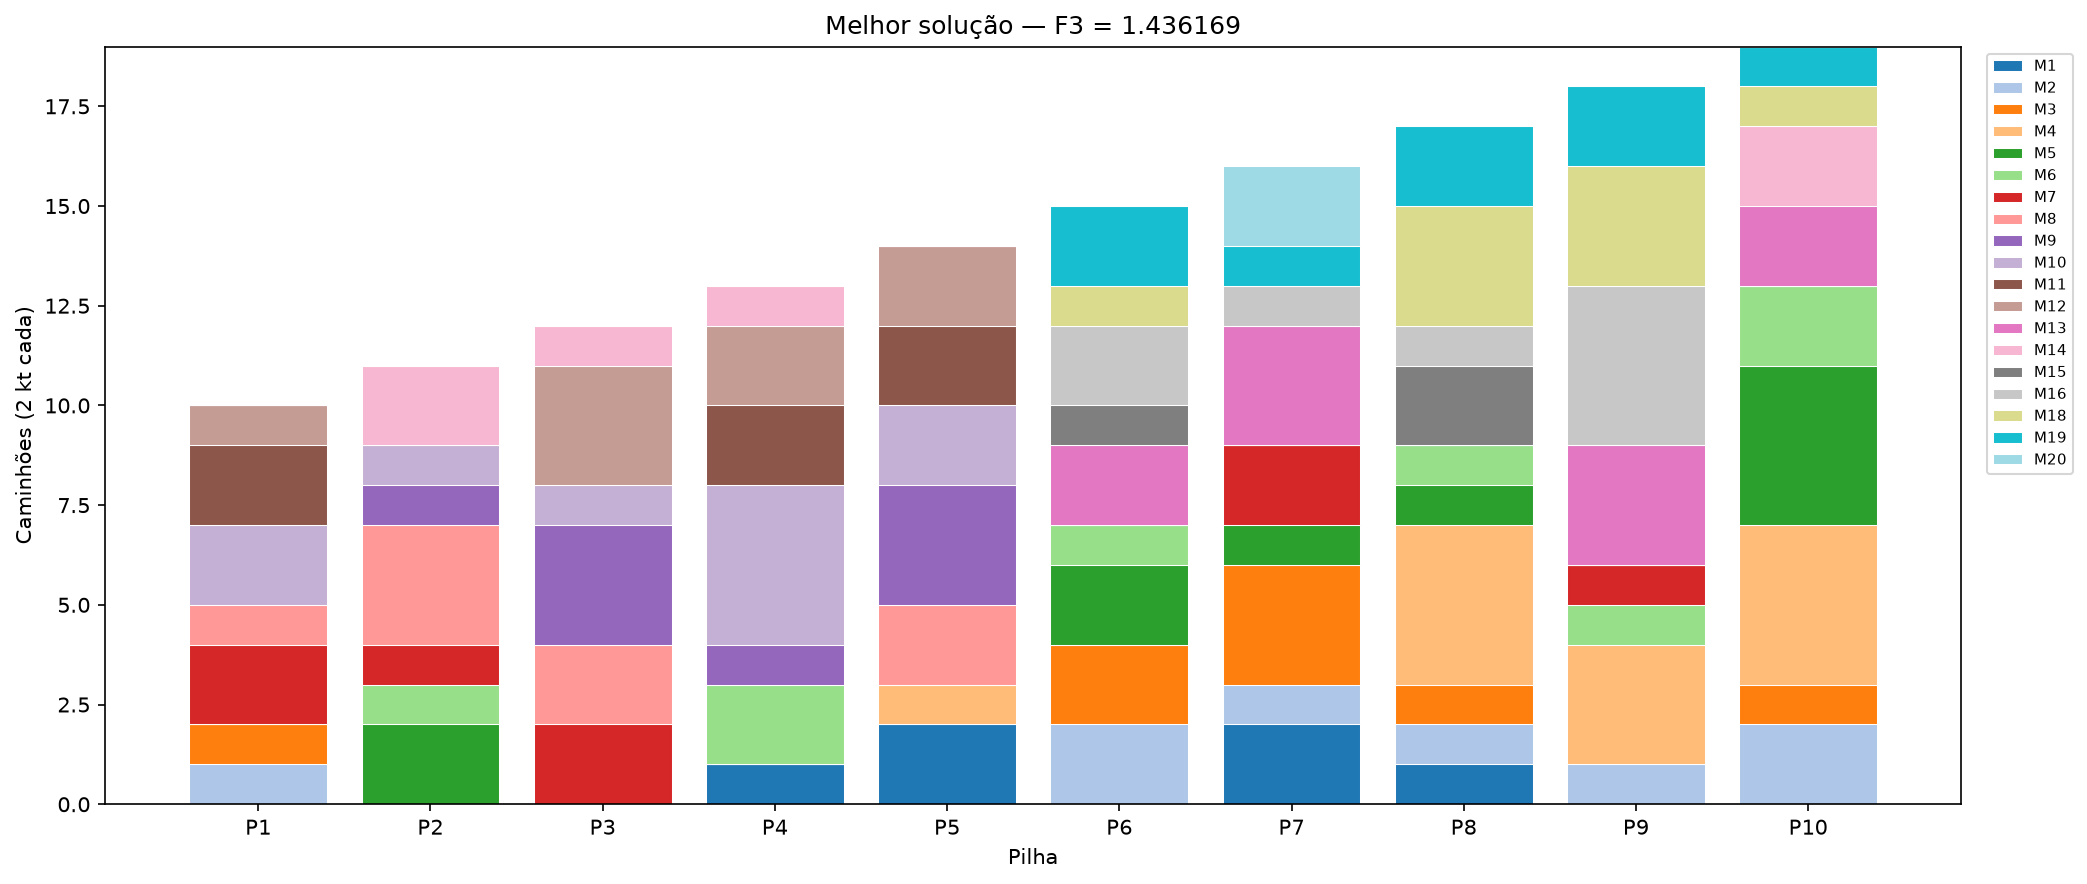
\includegraphics[width=\textwidth]{results/tp1_corrigido/melhor_solucao_f3.png}

\caption{Melhor composição para $f_3=\num{1.436169}$ (seed 789)}

\label{fig:sol_f3}

\end{figure}

\begin{table}[H]\centering\small

\caption{Matriz cruzada das melhores soluções mono-objetivo}

\begin{tabular}{lrrr}\toprule

Objetivo otimizado & $f_1$ (R\$) & $f_2$ (p.p.$^2$) & $f_3$ (p.p.$^2$) \\ \midrule

$f_1$ & \num{60300000} & \num{6.410508} & \num{5.995129} \\

$f_2$ & \num{63440000} & \num{2.372757} & \num{3.665272} \\

$f_3$ & \num{65740000} & \num{5.955709} & \num{1.436169} \\

\bottomrule\end{tabular}\end{table}

A matriz evidencia que os desempenhos devem ser comparados na mesma composição. O mínimo de cada coluna da tabela das cinco rodadas pertence a uma otimização independente; combinar esses três mínimos não define uma receita realizável. A matriz cruzada conserva os três valores de cada alternativa.

\subsection{Referências para a próxima etapa}

Os extremos abaixo são calculados sobre os 15 vetores finais viáveis, incluindo os valores de cada objetivo nas buscas dos outros dois. São referências empíricas, não provas de ideal, nadir ou ótimo global.

\begin{table}[H]\centering\small

\caption{Extremos empíricos para normalização na Entrega 2}

\begin{tabular}{lrr}\toprule Objetivo & Mínimo observado & Máximo observado \\ \midrule

$f_1$ & \num{60300000} & \num{65840000} \\

$f_2$ & \num{2.372757} & \num{6.705745} \\

$f_3$ & \num{1.436169} & \num{5.995129} \\

\bottomrule\end{tabular}\end{table}

Cada extremo aponta ao identificador da execução e ao hash do arquivo que contém sua composição em \texttt{referencias\_tp1.json}. A próxima etapa aplicará a mesma transformação min--max nos dois métodos. Novas soluções poderão extrapolar o intervalo empírico; os valores não devem ser truncados.

\subsection{Análise da revisão}

O acompanhamento separado pode melhorar o retorno sem alterar a trajetória estocástica por fitness: candidatos viáveis anteriormente descartados como incumbentes agora continuam disponíveis. Por isso, diferenças em relação ao log histórico não são tratadas como erro de reprodução. A disponibilidade das 15 composições permite conferir cada uma das alegações de viabilidade.

$f_1$: coeficiente de variação amostral de \num{0.2720}\%.

$f_2$: coeficiente de variação amostral de \num{0.0229}\%.

$f_3$: coeficiente de variação amostral de \num{0.5013}\%.

Com cinco sementes, essa comparação é descritiva e não comprova superioridade estatística, otimalidade ou cobertura do espaço de soluções.

\section{Conclusão}

As 15 soluções finais foram validadas individualmente e por auditoria independente. A base mono-objetivo corrigida, com registros e referências empíricas rastreáveis, está pronta para a etapa multiobjetivo.




% Conteúdo de docs/tp2/METODOLOGIA_TP2.tex
% Parte cumulativa do relatório. Resultados oficiais inseridos após auditoria.
\section{Otimização Multiobjetivo}
\label{sec:multiobjetivo}

As buscas mono-objetivo fornecem referências para explorar compromissos entre
custo, desvio de $SiO_2$ e desvio de $Al_2O_3$. Nesta etapa são utilizados os
métodos soma ponderada e $\varepsilon$-restrito sobre os mesmos dados,
representação, construtiva e vizinhanças do problema original. Seja $X$ o
conjunto de composições que satisfazem integralidade, massas, compatibilidades,
disponibilidades e faixas químicas já formuladas. Ambos os métodos mantêm
todas essas restrições; as restrições agregadas de desvio não substituem as
faixas químicas individuais de cada pilha.

\subsection{Normalização com referências empíricas do TP1}

Seja $S_{\mathrm{ref}}$ o conjunto das 15 soluções finais viáveis das buscas
mono-objetivo corrigidas, com cinco sementes para cada objetivo. Os três
objetivos foram recalculados em cada uma dessas composições, incluindo os
valores cruzados dos objetivos que não eram o alvo da respectiva busca.
Para $j\in\{1,2,3\}$, adotam-se
\begin{align}
 a_j &= \min_{x\in S_{\mathrm{ref}}} f_j(x), &
 b_j &= \max_{x\in S_{\mathrm{ref}}} f_j(x), &
 g_j(x) &= \frac{f_j(x)-a_j}{b_j-a_j}.
\end{align}
Os valores $a_j$ e $b_j$ são extremos da amostra, não estimativas certificadas
do ideal ou do nadir global. Por isso, soluções posteriores podem apresentar
$g_j<0$ ou $g_j>1$; esses valores são mantidos sem truncamento. A implementação
rejeita referências não finitas ou com amplitude degenerada. Todas as
configurações e repetições utilizam a mesma referência congelada, com origem
das composições e identificador de integridade no arquivo de referência.

\begin{table}[H]
\centering
\caption{Extremos empíricos usados na normalização. Valores exibidos arredondados;
os cálculos utilizam a precisão completa da referência armazenada.}
\label{tab:referencias_tp2}
\begin{tabular}{lrr}
\toprule
Objetivo & $a_j$ & $b_j$ \\
\midrule
$f_1$ (R\$) & \num{60300000} & \num{65840000} \\
$f_2$ (p.p.$^2$) & \num{2.3727567955} & \num{6.7057453980} \\
$f_3$ (p.p.$^2$) & \num{1.4361688772} & \num{5.9951294968} \\
\bottomrule
\end{tabular}
\end{table}

\subsection{Formulação por soma ponderada}

Para cada vetor de pesos $w$, resolve-se heuristicamente
\begin{equation}
 (P_w)\qquad \min_{x\in X}\;\sum_{j=1}^{3}w_jg_j(x),
 \qquad w_j\geq 0,\quad \sum_{j=1}^{3}w_j=1.
\end{equation}
A malha contém os 15 vetores $(i/4,j/4,k/4)$ com $i,j,k$ inteiros não
negativos e $i+j+k=4$, acrescidos do centro $(1/3,1/3,1/3)$. Assim, cada
varredura resolve 16 configurações, incluindo os três vértices, preferências
intermediárias e pesos iguais. A resolução é uma escolha operacional para
explorar diferentes compromissos com esforço finito, e não uma exigência
numérica do enunciado. Pesos não normalizam os objetivos por si mesmos e não
substituem a verificação de viabilidade. Soma ponderada e GVNS não asseguram
a recuperação de toda a fronteira de um problema discreto.

\subsection{Formulação por $\varepsilon$-restrito}

O custo normalizado é mantido como objetivo principal:
\begin{equation}
 (P_{\varepsilon})\qquad
 \min_{x\in X}\;g_1(x)\quad
 \text{sujeito a}\quad g_2(x)\leq\varepsilon_2,\quad
 g_3(x)\leq\varepsilon_3.
\end{equation}
Cada limite pertence a $\{0,1/3,2/3,1\}$, de modo que são resolvidos todos
os 16 pares do produto cartesiano, não apenas os quatro pares da diagonal.
A malha varia independentemente os dois limites de qualidade agregada.
Um limite normalizado zero corresponde ao mínimo empírico do respectivo
desvio no TP1, e não a desvio bruto nulo. Tetos iguais a um também não
eliminam as restrições físicas, nem tornam o subproblema automaticamente viável.

\subsection{Comparação, inviabilidade e observação dos candidatos}

O núcleo comum utiliza avaliação lexicográfica para ambos os métodos TP2.
Candidatos estruturalmente inválidos são rejeitados antes do cálculo dos
objetivos. Entre candidatos estruturalmente válidos, a comparação prioriza
viabilidade, violação agregada, escalar e desempate determinístico.
A violação química soma os quadrados dos excessos além da tolerância,
divididos pela amplitude da respectiva faixa. No método $\varepsilon$-restrito,
somam-se também os excessos positivos dos dois limites normalizados.
Qualidade e restrições $\varepsilon$ usam tolerância absoluta $10^{-9}$;
a soma dos pesos é validada com tolerância absoluta $10^{-12}$.

Na soma ponderada, o desempate utiliza $(\sum_jg_j,g_1,g_2,g_3)$.
No $\varepsilon$-restrito, utiliza $(g_2+g_3,g_2,g_3)$, sem compensar
uma piora no custo principal. Empate completo mantém a incumbente.
Essa regra TP2 é distinta da penalidade histórica preservada para reprodução
do TP1: multiplicadores de penalidade não são referências de normalização.

A trajetória aceita, a melhor viável do subproblema e o arquivo não dominado
são objetos distintos. Cada candidato avaliado é observado antes do filtro
de aceitação, inclusive se for rejeitado ou se encerrar o orçamento. A melhor
viável é atualizada separadamente. A ausência de uma solução viável encontrada
é registrada explicitamente e não constitui prova de inviabilidade matemática.

\subsection{Integração do GVNS e critérios de parada}

\begin{algorithm}[H]
\caption{GVNS escalar com observação e orçamento comum}
\label{alg:gvns_multiobjetivo}
\begin{algorithmic}[1]
\Require Configuração escalar, referência congelada, semente e limites
\State Inicializar RNG próprio e contadores; melhor viável $\gets\varnothing$
\State Gerar, avaliar e observar a solução construtiva como incumbente
\While{há orçamento e os critérios externos permitem continuar}
  \State $k\gets1$; registrar se houve melhoria da incumbente
  \While{$k\leq K_{\max}$ e há orçamento}
    \State Perturbar a incumbente com SHAKE, observando cada avaliação
    \State Aplicar VND com N1/N2/N3 e comparar pela chave lexicográfica
    \If{o resultado melhora estritamente a incumbente}
      \State Atualizar incumbente; $k\gets1$
    \Else
      \State $k\gets k+1$
    \EndIf
  \EndWhile
  \State Atualizar histórico e contador de iterações sem melhoria
\EndWhile
\State \Return Melhor viável observada, ou ausência explícita, e registros
\end{algorithmic}
\end{algorithm}

O orçamento inclui a avaliação inicial e avaliações repetidas, inclusive
dentro de SHAKE e VND. Tentativas estruturalmente inválidas são contabilizadas
separadamente. O VND retorna à primeira vizinhança após melhoria enquanto
dispõe dos cinco reinícios; depois disso, permanece na vizinhança atual
enquanto houver melhoria e avança quando não há melhoria. O limite não
equivale a cinco melhorias totais.

Os parâmetros de referência são 200 iterações externas, 60 sem melhoria,
$K_{\max}=3$, 20 amostras e cinco reinícios VND. O piloto utiliza teto de
\num{10000} avaliações por subproblema para avaliar tempo e viabilidade.
Após o piloto, foi mantido o teto de \num{10000} avaliações por run,
registrado no protocolo antes do início da campanha oficial. As 32 buscas
ponderadas do piloto encontraram viável; no $\varepsilon$-restrito, foram
18 de 32, com as ausências concentradas nos mesmos sete pares mais apertados
nas duas sementes. Esses resultados e o tempo de execução fundamentaram
a decisão de orçamento; não demonstram inviabilidade matemática desses pares.
Os dados piloto permanecem separados dos resultados oficiais.
Os dois métodos recebem o mesmo teto;
o esforço efetivamente utilizado e o motivo de parada são registrados.

\subsection{Repetições, arquivo não dominado e reprodutibilidade}

Uma execução de uma configuração é denominada \emph{run}; uma varredura
percorre as 16 configurações de uma abordagem. O desenho oficial contém
cinco varreduras por método, identificadas pelas sementes-base
$42,123,456,789,1011$, totalizando $2\times5\times16=160$ runs.
Cada combinação de base, método e configuração recebe uma semente efetiva
derivada por SHA-256, evitando dependência da ordem de execução. O piloto
utiliza bases externas $90001$ e $90002$ e saída própria, sem misturar seus
dados com a coleta oficial.

O arquivo usa dominância estrita de Pareto nos três objetivos brutos:
$x$ domina $y$ quando $f_j(x)\leq f_j(y)$ para todo $j$, com desigualdade
estrita em pelo menos um objetivo. A filtragem ocorre em 3D antes das
projeções. Composições físicas iguais agregam todas as suas origens;
composições distintas com vetor igual podem permanecer. Arquivos separados
por repetição permitem examinar variabilidade, enquanto a união filtrada
por método reúne as alternativas não dominadas encontradas em suas varreduras.
Nenhum desses arquivos certifica a fronteira global.

As seis projeções requeridas são $f_1\times f_2$, $f_1\times f_3$ e
$f_2\times f_3$ para cada método. Cores e símbolos identificam as repetições,
com escalas comuns entre métodos para cada objetivo. As tabelas devem
contabilizar todas as runs, inclusive aquelas sem viável encontrada.

Manifestos registram dados, referência, configuração, fontes, versões e seeds.
A retomada revalida runs completas antes de reutilizá-las e recomeça uma run
interrompida; arquivos temporários não representam conclusão. O verificador
independente recalcula objetivos, restrições e proveniência das composições
e recompõe os arquivos não dominados. Alterações incompatíveis exigem uma
campanha em diretório novo. A análise comparativa final depende da auditoria
da coleta oficial; a integração reduzida demonstra funcionamento, não
superioridade experimental de uma abordagem.




% Conteúdo de results/tp2/resultados_tp2.tex
% Gerado de produtos auditados por relatorio_tp2.py.
\section{Resultados da Otimização Multiobjetivo}
\label{sec:resultados_tp2}
A coleta reuniu 160 buscas, com 5 varreduras por abordagem. Todas as buscas, inclusive as que não encontraram viável, permanecem contabilizadas. A auditoria recalculou objetivos e restrições das composições, verificou proveniência e recompôs os arquivos em 3D.
\begin{table}[H]\centering\small
\caption{Contabilidade das buscas e uniões não dominadas por método.}
\label{tab:tp2_metodos}
\begin{tabular}{lrrrrr}\toprule
Método & Runs & Viáveis & Sem viável & Composições ND & Vetores ND \\ \midrule
Soma ponderada & 80 & 80 & 0 & 3961 & 3830 \\
$\varepsilon$-restrito & 80 & 45 & 35 & 1206 & 1182 \\
\bottomrule\end{tabular}\end{table}

% Conteúdo de results/tp2/figuras/tabela_repeticoes.tex
% Gerado por figuras_tp2.py; não editar números manualmente.
\begin{table}[H]\centering
\caption{Resultados por varredura. ND: composições não dominadas em três objetivos.}
\label{tab:tp2_repeticoes}
\begin{tabular}{llrrrr}\toprule
Método & Semente-base & Runs & Viáveis & Sem viável & ND \\ \midrule
Ponderada & 42 & 16 & 16 & 0 & 1617 \\
Ponderada & 123 & 16 & 16 & 0 & 1963 \\
Ponderada & 456 & 16 & 16 & 0 & 1861 \\
Ponderada & 789 & 16 & 16 & 0 & 1744 \\
Ponderada & 1011 & 16 & 16 & 0 & 1954 \\
$\varepsilon$-restrito & 42 & 16 & 9 & 7 & 657 \\
$\varepsilon$-restrito & 123 & 16 & 9 & 7 & 790 \\
$\varepsilon$-restrito & 456 & 16 & 9 & 7 & 674 \\
$\varepsilon$-restrito & 789 & 16 & 9 & 7 & 634 \\
$\varepsilon$-restrito & 1011 & 16 & 9 & 7 & 741 \\
\bottomrule\end{tabular}
\end{table}


\begin{table}[H]\centering\small
\caption{Intervalos dos três objetivos nas uniões ND. Extremos de objetivos diferentes podem pertencer a composições diferentes.}
\label{tab:tp2_intervalos}
\resizebox{\linewidth}{!}{\begin{tabular}{lrrr}\toprule
Método & Custo (milhões de R\$) & Desvio $SiO_2$ (p.p.$^2$) & Desvio $Al_2O_3$ (p.p.$^2$) \\ \midrule
Soma ponderada & \num{60.740} -- \num{65.680} & \num{2.407} -- \num{6.872} & \num{1.452} -- \num{5.442} \\
$\varepsilon$-restrito & \num{60.460} -- \num{64.520} & \num{3.039} -- \num{6.616} & \num{2.325} -- \num{5.822} \\
\bottomrule\end{tabular}}\end{table}
\begin{table}[H]\centering\small
\caption{Exemplos de composições efetivamente encontradas nos extremos marginais de cada método. Cada linha é uma alternativa completa, não uma combinação de mínimos.}
\label{tab:tp2_extremos}
\begin{tabular}{llrrr}\toprule
Método & Extremo & Custo (milhões R\$) & $f_2$ (p.p.$^2$) & $f_3$ (p.p.$^2$) \\ \midrule
Soma ponderada & $f_1$ mínimo & \num{60.740} & \num{6.625} & \num{4.959} \\
Soma ponderada & $f_2$ mínimo & \num{63.700} & \num{2.407} & \num{3.284} \\
Soma ponderada & $f_3$ mínimo & \num{65.660} & \num{5.498} & \num{1.452} \\
$\varepsilon$-restrito & $f_1$ mínimo & \num{60.460} & \num{6.343} & \num{5.706} \\
$\varepsilon$-restrito & $f_2$ mínimo & \num{63.120} & \num{3.039} & \num{3.640} \\
$\varepsilon$-restrito & $f_3$ mínimo & \num{64.460} & \num{3.783} & \num{2.325} \\
\bottomrule\end{tabular}\end{table}
\begin{table}[H]\centering\small
\caption{Esforço efetivo. Tempos de busca são decorridos, não de CPU, e excluem persistência, consolidação e auditoria.}
\label{tab:tp2_esforco}
\begin{tabular}{lrrr}\toprule
Método & Avaliações & Tempo de busca (s) & Média por run (s) \\ \midrule
Soma ponderada & \num{800000} & \num{955.32} & \num{11.94} \\
$\varepsilon$-restrito & \num{800000} & \num{881.86} & \num{11.02} \\
\bottomrule\end{tabular}\end{table}
A coleta completa, incluindo persistência e consolidação, levou \num{46.01} minutos. A auditoria e geração de figuras consumiram \num{13.29} minutos adicionais. Esses valores não se confundem com a soma dos tempos dos solvers.
\subsection{Projeções e variabilidade entre varreduras}
As figuras mantêm os arquivos ND de cada repetição antes da projeção. Um ponto aparentemente dominado em 2D pode permanecer não dominado em 3D. A mesma composição pode aparecer nas cinco varreduras, com todas as origens preservadas.
\begin{figure}[H]\centering
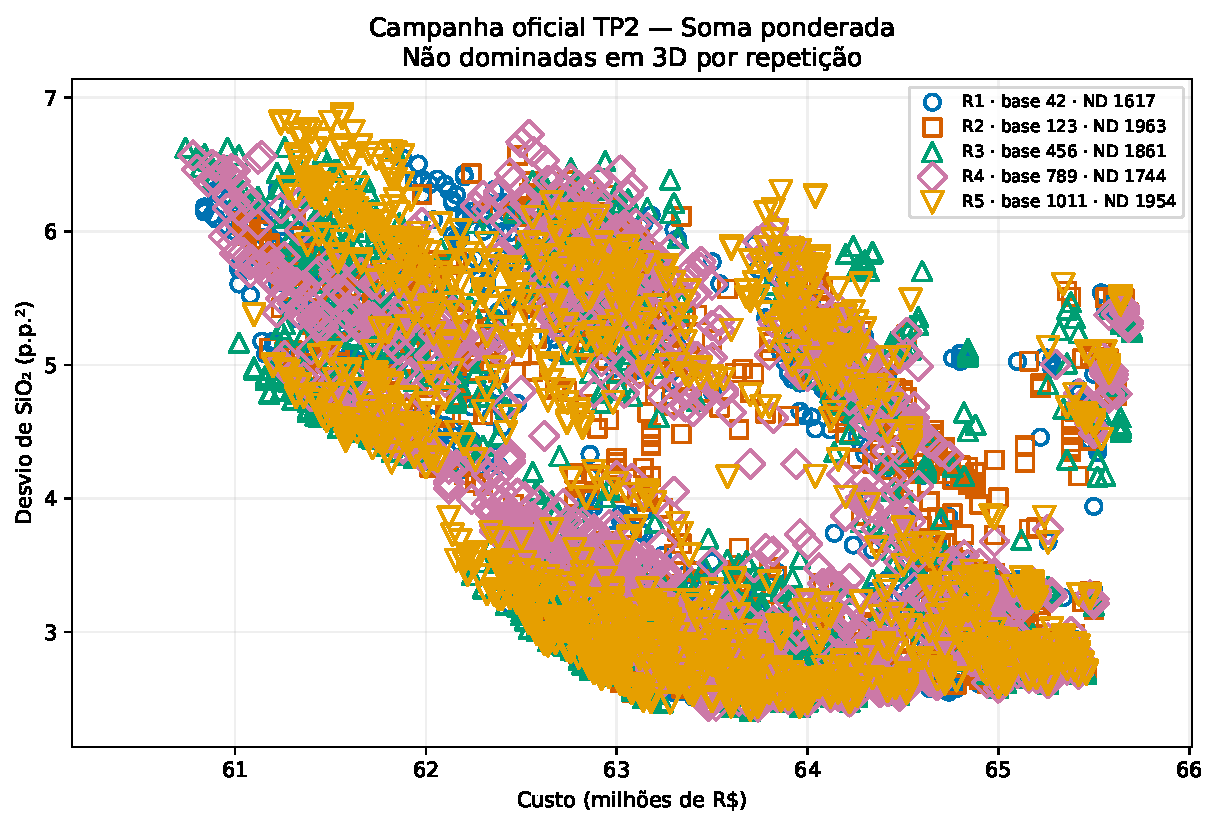
\includegraphics[width=0.88\linewidth]{results/tp2/figuras/ponderada_f1_f2.pdf}
\caption{Soma ponderada: projeção $f_1\times f_2$, com as repetições identificadas.}
\label{fig:tp2_ponderada_1_2}
\end{figure}
\begin{figure}[H]\centering
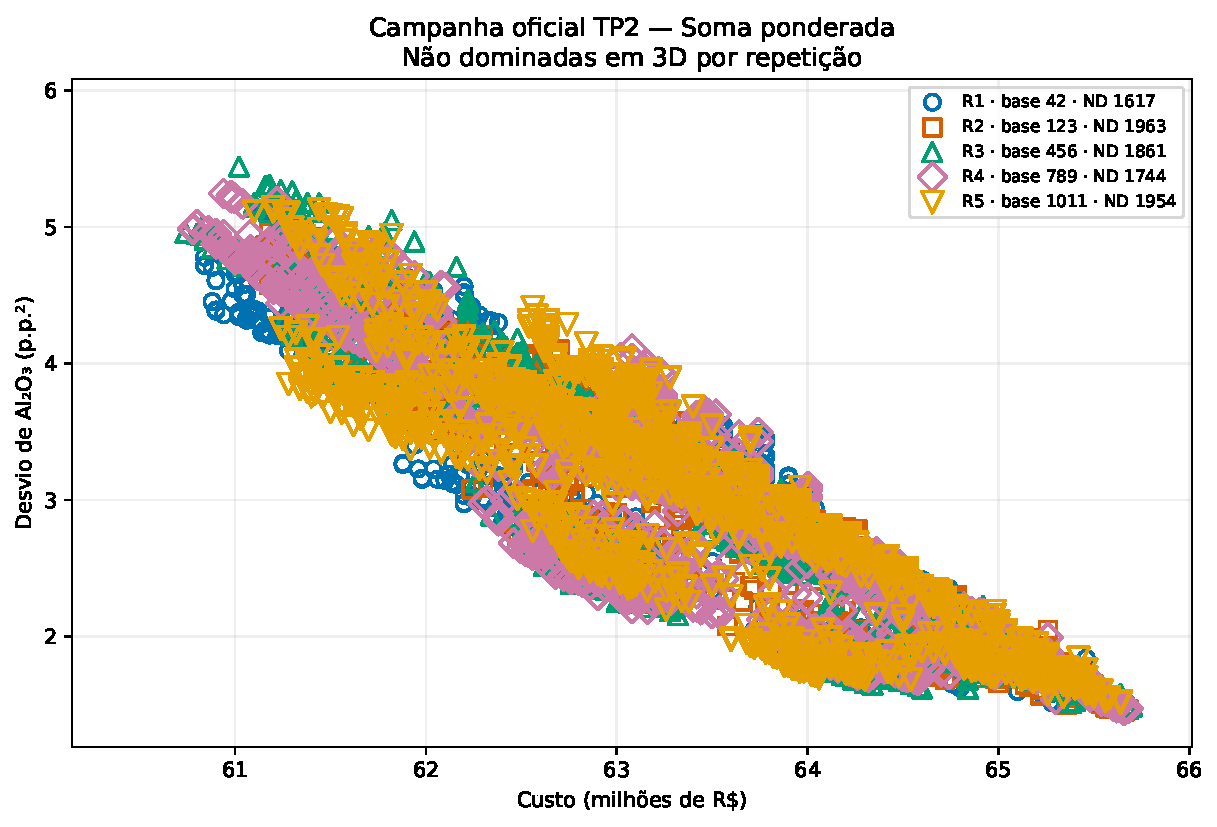
\includegraphics[width=0.88\linewidth]{results/tp2/figuras/ponderada_f1_f3.pdf}
\caption{Soma ponderada: projeção $f_1\times f_3$, com as repetições identificadas.}
\label{fig:tp2_ponderada_1_3}
\end{figure}
\begin{figure}[H]\centering
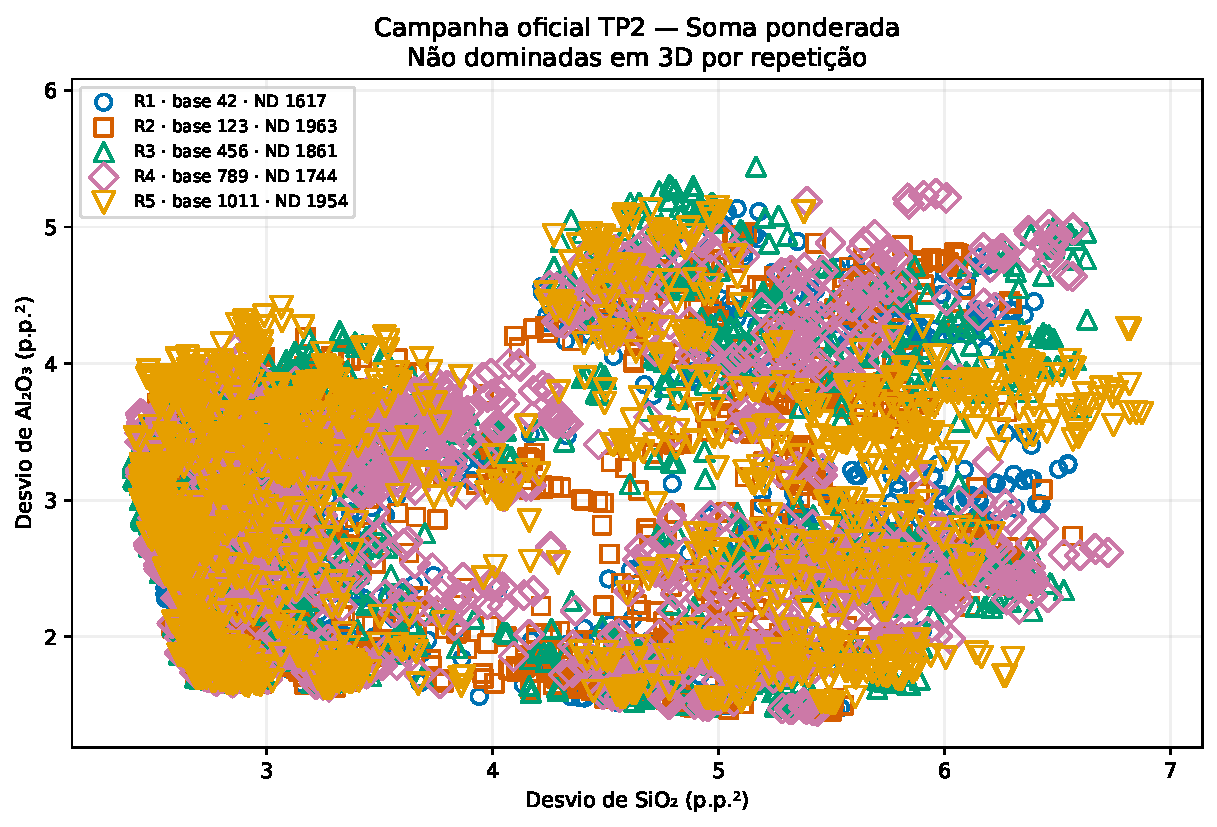
\includegraphics[width=0.88\linewidth]{results/tp2/figuras/ponderada_f2_f3.pdf}
\caption{Soma ponderada: projeção $f_2\times f_3$, com as repetições identificadas.}
\label{fig:tp2_ponderada_2_3}
\end{figure}
\begin{figure}[H]\centering
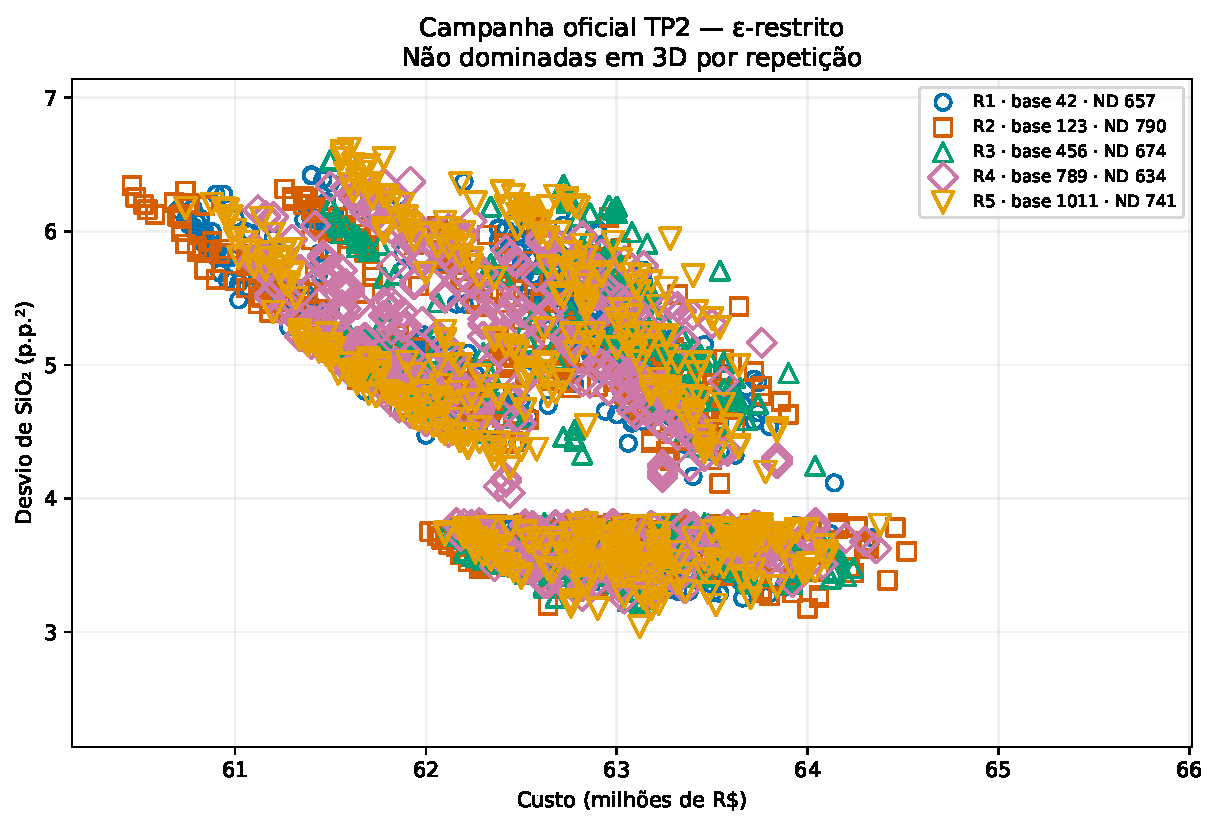
\includegraphics[width=0.88\linewidth]{results/tp2/figuras/epsilon_f1_f2.pdf}
\caption{$\varepsilon$-restrito: projeção $f_1\times f_2$, com as repetições identificadas.}
\label{fig:tp2_epsilon_1_2}
\end{figure}
\begin{figure}[H]\centering
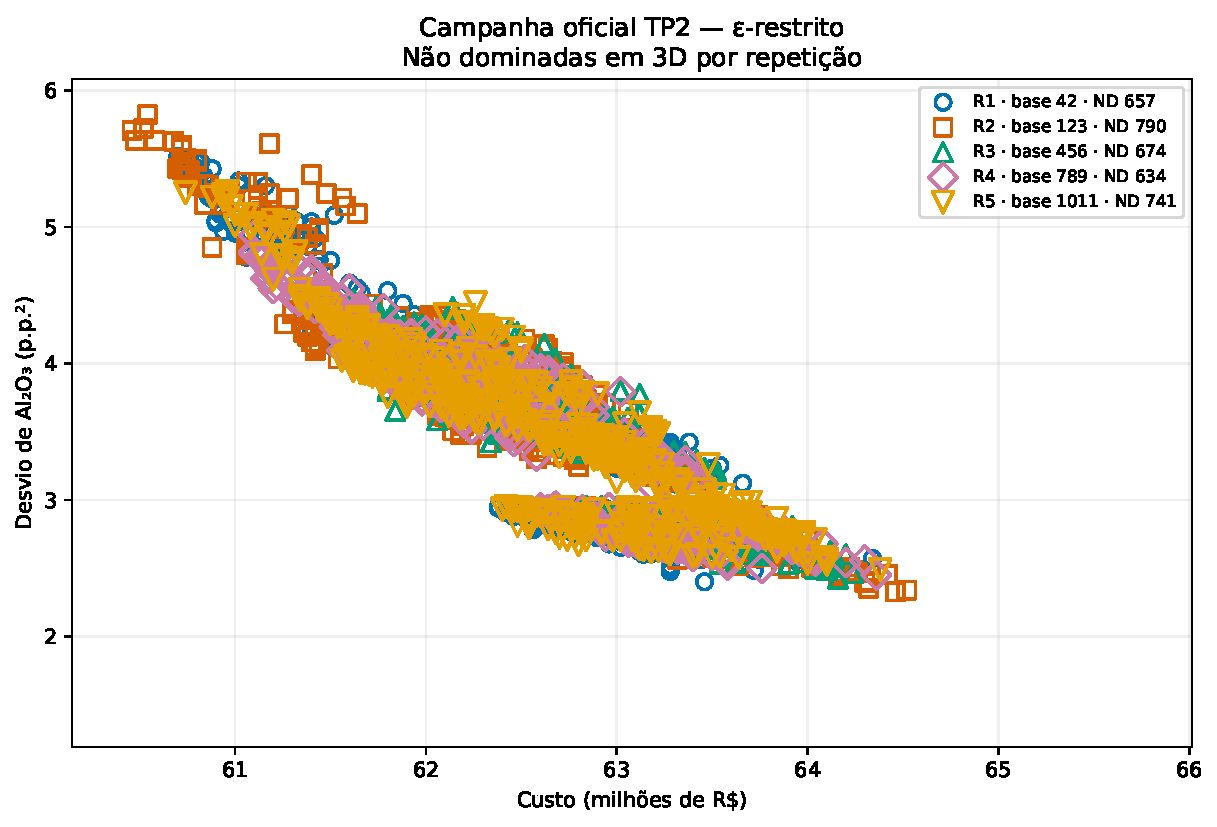
\includegraphics[width=0.88\linewidth]{results/tp2/figuras/epsilon_f1_f3.pdf}
\caption{$\varepsilon$-restrito: projeção $f_1\times f_3$, com as repetições identificadas.}
\label{fig:tp2_epsilon_1_3}
\end{figure}
\begin{figure}[H]\centering
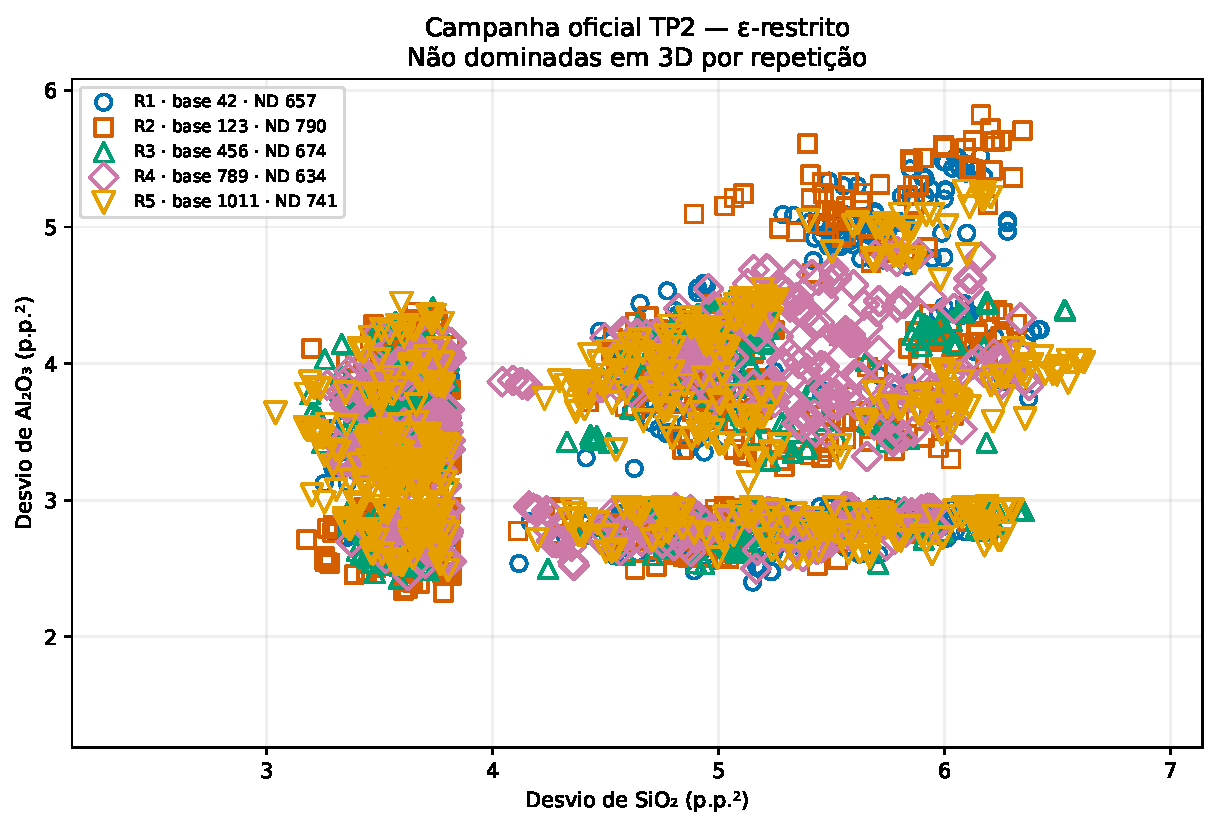
\includegraphics[width=0.88\linewidth]{results/tp2/figuras/epsilon_f2_f3.pdf}
\caption{$\varepsilon$-restrito: projeção $f_2\times f_3$, com as repetições identificadas.}
\label{fig:tp2_epsilon_2_3}
\end{figure}
\subsection{Comparação descritiva das aproximações}
Entre os vetores distintos encontrados, a união ponderada domina estritamente \num{66.24}\% dos vetores da união $\varepsilon$-restrita; no sentido inverso, a fração é \num{3.26}\%. Essa comparação usa três objetivos e apenas as amostras encontradas; não certifica superioridade global dos métodos.
Há 0 vetores de objetivos iguais e 0 composições físicas comuns entre as uniões. Essas contagens são distintas da quantidade de pontos sobrepostos em uma projeção.
O escalar principal não é comparável entre métodos ou configurações. A comparação deve considerar os três objetivos brutos, as mesmas referências, o teto comum e o esforço efetivamente realizado. Mais composições no arquivo não provam melhor método. As cinco varreduras, e não as buscas individuais, representam as repetições do desenho.




% Conteúdo de docs/tp2/DISCUSSAO_TP2.tex
% Discussão da campanha oficial integralmente auditada.
\subsection{Compromissos observados entre custo e qualidade}

Na amostra obtida, o $\varepsilon$-restrito alcançou o menor custo,
R\$~\num{60460000}, enquanto a soma ponderada atingiu os menores desvios
de $SiO_2$ e $Al_2O_3$, respectivamente \num{2.406656} e \num{1.452043}
p.p.$^2$. Esses extremos não constituem uma única solução ideal. As
alternativas completas que os originaram estão na
Tabela~\ref{tab:tp2_extremos}, com composições e proveniência recuperáveis
no conjunto de dados.

Por exemplo, a alternativa de menor custo do $\varepsilon$-restrito
apresenta o vetor, com custo em milhões de reais,
$(\num{60.460},\num{6.343},\num{5.706})$. A alternativa ponderada de menor
desvio de $SiO_2$ tem vetor
$(\num{63.700},\num{2.407},\num{3.284})$.
Nesse par, um acréscimo de R\$~\num{3240000} reduz ambos os desvios,
evidenciando o compromisso entre economia e qualidade.

A alternativa ponderada de menor desvio de $Al_2O_3$ tem vetor
$(\num{65.660},\num{5.498},\num{1.452})$.
Em relação à alternativa ponderada de menor desvio de $SiO_2$, custa
R\$~\num{1960000} a mais, melhora $Al_2O_3$ e piora $SiO_2$.
Portanto, o conflito também ocorre entre as duas medidas de qualidade,
não apenas entre custo e um indicador agregado.

O mínimo individual corrigido do TP1 para custo foi R\$~\num{60300000}.
Para os desvios de $SiO_2$ e $Al_2O_3$, os mínimos foram, respectivamente,
\num{2.372757} e \num{1.436169} p.p.$^2$. A coleta multiobjetivo não
superou esses três mínimos marginais; sua finalidade é explorar
compromissos, e não repetir a otimização isolada de cada objetivo.
Também foi encontrado $f_2$ de \num{6.872459} p.p.$^2$ na união ponderada,
acima do máximo empírico TP1 de \num{6.705745}; o valor normalizado é
aproximadamente \num{1.038}. Isso é permitido pela normalização sem
truncamento e não implica violar as restrições físicas.

\subsection{Semelhança e variabilidade entre as cinco varreduras}

As cinco varreduras ponderadas encontraram intervalos marginais bastante
semelhantes. Entre os dez pares de varreduras, a menor razão entre o
comprimento da interseção e o da união dos intervalos foi
\num{91.53}\% para custo, \num{91.42}\% para $SiO_2$ e \num{87.47}\%
para $Al_2O_3$. No $\varepsilon$-restrito, esses mínimos foram
\num{67.49}\%, \num{87.32}\% e \num{58.39}\%, respectivamente.
A medida é apenas descritiva e marginal: não demonstra que as composições
ou a distribuição dos pontos em 3D sejam iguais.

Nas seis projeções das Figuras~\ref{fig:tp2_ponderada_1_2}
a~\ref{fig:tp2_epsilon_2_3}, as cores e símbolos das cinco repetições
ocupam faixas amplamente sobrepostas dentro de cada abordagem. A projeção
custo versus $Al_2O_3$ mostra bandas decrescentes comuns às repetições;
na projeção das duas qualidades, observam-se agrupamentos e lacunas,
sobretudo no $\varepsilon$-restrito. Assim, as repetições alcançaram regiões
projetadas semelhantes, com diferenças de extensão e densidade local,
sem evidência de identidade entre os conjuntos tridimensionais.

Os arquivos por repetição contêm de \num{1617} a \num{1963} composições
ponderadas e de \num{634} a \num{790} composições $\varepsilon$-restritas
ND. Assim, contagens diferentes coexistem com intervalos sobrepostos;
uma varredura com mais composições não necessariamente amplia a região
de objetivos alcançada. As projeções identificam a distribuição de cada
repetição; a união por método preserva a proveniência e filtra novamente
em três objetivos.

Em todas as sementes, as 16 configurações ponderadas encontraram viável,
enquanto nove dos 16 pares $\varepsilon$ encontraram viável. As 35 ausências
se concentram nos sete pares com pelo menos um limite normalizado zero:
$(0,0)$, $(0,1/3)$, $(0,2/3)$, $(0,1)$, $(1/3,0)$, $(2/3,0)$ e $(1,0)$.
Esse padrão sugere dificuldade persistente da busca em alcançar os
extremos empíricos de qualidade sob os limites simultâneos. Não demonstra
que esses subproblemas sejam matematicamente inviáveis, nem autoriza
substituir as sementes por repetições bem-sucedidas.

\subsection{Limitações e implicações para a continuidade}

A soma ponderada produziu maior cobertura descritiva da amostra oposta,
conforme a comparação bidirecional em três objetivos, e alcançou extremos
de qualidade mais próximos dos resultados mono-objetivo. O
$\varepsilon$-restrito forneceu o menor custo e alternativas que não são
todas dominadas pela união ponderada. As duas amostras contribuem para
explicitar preferências diferentes; cardinalidade, mínimos marginais e
cobertura devem ser considerados em conjunto.

As conclusões se restringem à instância, ao GVNS, às duas malhas e ao teto
de \num{10000} avaliações por configuração. Malhas finitas podem omitir
regiões relevantes; a escalarização ponderada não recupera necessariamente
toda a fronteira de um problema discreto. O orçamento e as sementes
limitam a exploração, e o arquivo contém apenas soluções observadas pela
heurística. Não se dispõe de prova de otimalidade ou de completude da
fronteira. A comparação de tempos é descritiva, com custo adicional de
observação, persistência, consolidação e auditoria explicitado no protocolo.

\section{Considerações Finais da Entrega 2}

Foram integradas duas formulações escalares normalizadas ao GVNS existente,
com orçamento comum, cinco varreduras por abordagem, preservação da melhor
viável e dos candidatos não dominados, registros completos e verificação
independente. As seis projeções e as tabelas permitem examinar custo,
qualidades e variabilidade sem substituir a comparação tridimensional por
dominância aparente em duas dimensões.

A escolha de uma ação final permanece para a etapa multicritério seguinte.
As composições e suas origens foram preservadas para permitir recuperar os
três objetivos e calcular atributos adicionais sem reconstruir receitas
a partir de gráficos ou valores arredondados.



\clearpage

% Conteúdo de decisao_tp3.tex
\section{Tomada de decisão multicritério}

\subsection{Da otimização à escolha de uma composição}

A etapa mono-objetivo isolou os melhores desempenhos de custo e qualidade e forneceu referências empíricas para o GVNS multiobjetivo. Na segunda etapa, a Soma Ponderada e o \(\varepsilon\)-restrito geraram composições com compromissos diferentes entre custo e desvios químicos. Nesta etapa, as mesmas composições são avaliadas também pela uniformidade das receitas, para selecionar um plano de formação das dez pilhas.

A consolidação partiu das duas uniões oficiais, com 3.961 composições da Soma Ponderada e 1.206 do \(\varepsilon\)-restrito. A identidade de uma composição é dada pela contagem de caminhões de cada minério em cada pilha. A ordem dos caminhões é ignorada, e a origem das alternativas é preservada. Foram obtidas 5.167 composições distintas. Após calcular o quarto critério, o filtro de dominância manteve 4.327 alternativas para ambos os métodos.

Uma composição foi descartada quando outra apresentou valor menor ou igual nos quatro critérios e estritamente menor em pelo menos um. O filtro foi aplicado após o cálculo da uniformidade, de modo que uma receita pudesse permanecer elegível por sua vantagem operacional. A análise se restringe às composições armazenadas nas duas uniões da Entrega 2 e à instância estudada.

\subsection{Variação da receita por equipamento}

Para a pilha j, seja x\textsubscript{i}\textsubscript{j} a quantidade de caminhões do minério i. Como cada caminhão transporta 2 kt, a fração em massa p\textsubscript{i}\textsubscript{j} é a razão entre x\textsubscript{i}\textsubscript{j} e o total de caminhões da pilha. Para cada Sinter k, calcula-se a receita média dos integrantes do seu conjunto de pilhas J\textsubscript{k}. A receita média atribui o mesmo peso a cada pilha, ainda que suas massas totais sejam diferentes.

\[p_{ij}=\frac{x_{ij}}{\sum_h x_{hj}},\qquad \bar p_{ik}=\frac{1}{|J_k|}\sum_{j\in J_k}p_{ij}.\]

\[f_4=\frac{D_1+D_2}{2},\qquad D_k=\frac{1}{2|J_k|}\sum_{j\in J_k}\sum_i|p_{ij}-\bar p_{ik}|.\]

O fator 1/2 transforma a soma das diferenças absolutas em distância de variação total. O resultado é expresso como porcentagem no relatório, e zero representa receitas idênticas dentro de cada equipamento. A medida usa as proporções dos insumos. Duas pilhas podem apresentar teores químicos próximos e, ainda assim, depender de receitas distintas para atingi-los.

\clearpage

\subsection{Parâmetros de referência e métodos}

Os quatro critérios são de minimização. O cenário-base usa pesos iguais de 25\% como referência transparente, dado que o case não fornece uma hierarquia operacional validada entre os quatro atributos. A matriz de critérios do AHP contém apenas valores 1, e os pesos derivados são usados também no PROMETHEE II. As preferências são hipóteses de decisão da instância, avaliadas por sensibilidade.

Para cada critério j, o desempenho x\textsubscript{j} é normalizado em z\textsubscript{j} entre o mínimo e o máximo observados nas alternativas retidas. Menor valor é preferível. Um critério constante recebe z\textsubscript{j} = 0 para todas as alternativas. Os limites desta etapa são calculados sobre as alternativas de decisão, enquanto a normalização da Entrega 2 usou as referências empíricas mono-objetivo.

\[z_j(a)=\frac{x_j(a)-\min_b x_j(b)}{\max_b x_j(b)-\min_b x_j(b)}.\]

No AHP (Saaty, 2008), o autovetor principal da matriz recíproca de critérios é normalizado para obter os pesos. No cenário-base, \(\lambda\)máx = 4 e a razão de consistência é zero. A avaliação das alternativas usa o modo ideal com a escala quantitativa s\textsubscript{j}(a) = 5^(-z\textsubscript{j}(a)). As comparações de cada critério são dadas pelas razões s\textsubscript{j}(a)/s\textsubscript{j}(b), cuja matriz é consistente por construção. A pontuação de cada composição é \(\sum\)\textsubscript{j} w\textsubscript{j} s\textsubscript{j}(a). A razão 5 entre o melhor e o pior desempenho fornece uma gradação contínua e constitui uma escolha de modelagem.

No PROMETHEE II (Brans, Vincke e Mareschal, 1986), para cada par (a,b), calcula-se d\textsubscript{j} = z\textsubscript{j}(b) - z\textsubscript{j}(a). A função de preferência linear vale zero para d\textsubscript{j} \(\leq\) q\textsubscript{j}, cresce como (d\textsubscript{j} - q\textsubscript{j})/(p\textsubscript{j} - q\textsubscript{j}) entre os limiares e vale 1 para d\textsubscript{j} \(\geq\) p\textsubscript{j}. O índice de preferência do par é a soma ponderada dessas preferências. Os fluxos positivo e negativo são as médias da preferência de a sobre as demais alternativas e das demais sobre a, respectivamente. Ordena-se pelo fluxo líquido, \(\phi\)\textsuperscript{+} - \(\phi\)\textsuperscript{-}.

No cenário-base, q = 5\% e p = 25\% da amplitude observada em cada critério. Esses valores oferecem uma faixa de diferenças desprezíveis e uma transição até a preferência plena sem assumir tolerâncias industriais que o case não informa. As diferenças nas unidades originais são apresentadas a seguir.

\begin{table}[H]
\centering
\small
\caption{Limiares do PROMETHEE II no cenário-base.}
\begin{tabular}{@{}p{0.374\linewidth}p{0.212\linewidth}p{0.264\linewidth}@{}}
\toprule
Critério & Indiferença (q) & Preferência plena (p) \\
\midrule
Custo (R\$) & 261.000 & 1.305.000 \\
Sílica (p.p.\textsuperscript{2}) & 0,223 & 1,116 \\
Alumina (p.p.\textsuperscript{2}) & 0,218 & 1,092 \\
Receita (p.p.) & 0,952 & 4,761 \\
\bottomrule
\end{tabular}
\end{table}

\clearpage

\subsection{Resultados do cenário-base}

A composição A01 (b47e00d37e63e5a7) foi a única primeira colocada em ambos os métodos. Sua prioridade AHP foi 0,746884, e seu fluxo líquido no PROMETHEE II foi 0,347997. A diferença de fluxo para a segunda colocada foi de aproximadamente 0,000110, o que motivou examinar a estabilidade da escolha antes de recomendar a receita.

A Tabela 12 apresenta os quatro critérios para todas as composições que chegaram ao topo em pelo menos um dos cenários analisados. A tabela integral das 4.327 alternativas avaliadas, com seus critérios, posições e pontuações no cenário-base, acompanha o relatório no arquivo matriz\_decisao\_tp3.csv.

\begin{table}[H]
\centering
\small
\caption{Critérios das alternativas que venceram em pelo menos um cenário.}
\begin{tabular}{@{}p{0.076\linewidth}p{0.230\linewidth}p{0.136\linewidth}p{0.136\linewidth}p{0.136\linewidth}p{0.136\linewidth}@{}}
\toprule
Ref. & ID da composição & Custo (R\$ mi) & Sílica (p.p.\textsuperscript{2}) & Alumina (p.p.\textsuperscript{2}) & Receita (\%) \\
\midrule
A01 & b47e00d37e63e5a7 & 65,26 & 2,760 & 1,801 & 24,31 \\
A02 & 5941e6243e7e796d & 62,28 & 3,475 & 4,274 & 26,13 \\
A03 & c131c7c9c53c5ad4 & 60,46 & 6,343 & 5,706 & 34,17 \\
A04 & fc32e80fa175f6df & 61,56 & 5,067 & 4,227 & 26,22 \\
A05 & f85f294dc3abfacd & 65,14 & 2,685 & 1,926 & 25,38 \\
A06 & d50023ef81ccd6e4 & 65,42 & 2,826 & 1,662 & 25,93 \\
A07 & d63557033bc83f00 & 65,40 & 2,718 & 1,740 & 25,41 \\
A08 & 00d66afb5bff1877 & 64,96 & 2,805 & 1,905 & 24,90 \\
A09 & 0113d1874f1c18e4 & 64,86 & 2,845 & 1,962 & 24,67 \\
A10 & 9be3e41e1a21bca8 & 62,86 & 2,791 & 3,675 & 27,22 \\
\bottomrule
\end{tabular}
\end{table}

Os métodos convergiram no cenário-base, embora produzam prioridades diferentes para o restante da lista. O AHP sintetiza prioridades locais por critério. O PROMETHEE II compara a intensidade das vantagens e desvantagens de cada alternativa em relação às demais, considerando os limiares.

Para empates em primeiro, propõe-se comparar primeiro a variação da receita, depois o custo, o desvio de sílica e o desvio de alumina, sempre em ordem crescente. Se todos os valores coincidirem, o menor ID estabelece uma ordem reprodutível. O cenário-base teve uma única vencedora por método e dispensou esse desempate. Quando métodos distintos indicam vencedoras diferentes sob outra preferência, a comparação deve explicitar qual compromisso operacional corresponde àquele cenário.

\clearpage

\subsection{Análise de sensibilidade}

Foram avaliados 20 cenários. Em nove deles, variaram-se os pesos com os limiares do cenário-base. Cada critério recebeu, isoladamente, 40\% ou 55\% do peso, e um cenário atribuiu 70\% aos dois critérios químicos em conjunto. Nos dez cenários de limiares, mantiveram-se os pesos iguais e aplicaram-se os pares (2\%, 15\%) ou (10\%, 40\%) a todos os critérios ou a um critério por vez.

\begin{table}[H]
\centering
\small
\caption{Vencedoras e posição da composição de referência A01.}
\begin{tabular}{@{}p{0.383\linewidth}p{0.119\linewidth}p{0.102\linewidth}p{0.136\linewidth}p{0.111\linewidth}@{}}
\toprule
Cenário & Vence AHP & Pos. A01 & Vence P. II & Pos. A01 \\
\midrule
Cenário-base & A01 & 1 & A01 & 1 \\
Custo com 40\% de peso & A01 & 1 & A02 & 629 \\
Custo com 55\% de peso & A03 & 938 & A04 & 3065 \\
Sílica com 40\% de peso & A01 & 1 & A01 & 1 \\
Sílica com 55\% de peso & A01 & 1 & A05 & 3 \\
Alumina com 40\% de peso & A01 & 1 & A01 & 1 \\
Alumina com 55\% de peso & A06 & 2 & A06 & 10 \\
Receita com 40\% de peso & A01 & 1 & A01 & 1 \\
Receita com 55\% de peso & A01 & 1 & A01 & 1 \\
Qualidade com 70\% de peso & A01 & 1 & A07 & 4 \\
Limiar menor · Todos & A01 & 1 & A07 & 4 \\
Limiar menor · Custo & A01 & 1 & A08 & 2 \\
Limiar menor · Sílica & A01 & 1 & A01 & 1 \\
Limiar menor · Alumina & A01 & 1 & A01 & 1 \\
Limiar menor · Receita & A01 & 1 & A08 & 2 \\
Limiar maior · Todos & A01 & 1 & A09 & 2 \\
Limiar maior · Custo & A01 & 1 & A08 & 3 \\
Limiar maior · Sílica & A01 & 1 & A09 & 3 \\
Limiar maior · Alumina & A01 & 1 & A10 & 4 \\
Limiar maior · Receita & A01 & 1 & A01 & 1 \\
\bottomrule
\end{tabular}
\end{table}

A01 manteve o primeiro lugar em sete das nove variações de pesos no AHP e em quatro no PROMETHEE II. Nas dez variações isoladas dos limiares, A01 venceu três vezes no PROMETHEE II. O AHP permaneceu igual nesses dez testes, pois os limiares pertencem ao PROMETHEE II. Essas contagens descrevem apenas os cenários testados.

\clearpage

\subsection{Recomendação e compromissos}

Recomenda-se A01 para o cenário de referência, em que o custo, a sílica, a alumina e a uniformidade da receita têm o mesmo peso. A composição custa R\$ 65,26 milhões, apresenta desvios quadráticos de 2,760 p.p.\textsuperscript{2} para SiO\textsubscript{2} e 1,801 p.p.\textsuperscript{2} para Al\textsubscript{2}O\textsubscript{3} e registra 24,31\% de variação de receita. É a menor variação observada no conjunto consolidado.

Com 40\% de peso para custo, o PROMETHEE II escolhe A02 (5941e6243e7e796d). A economia é de R\$ 2,98 milhões em relação a A01. Em contrapartida, os desvios de sílica e alumina passam de 2,760 e 1,801 para 3,475 e 4,274 p.p.\textsuperscript{2}, e a variação de receita sobe para 26,13\%. Com 55\% de peso para custo, os dois métodos deslocam A01 do topo.

\begin{figure}[H]
\centering
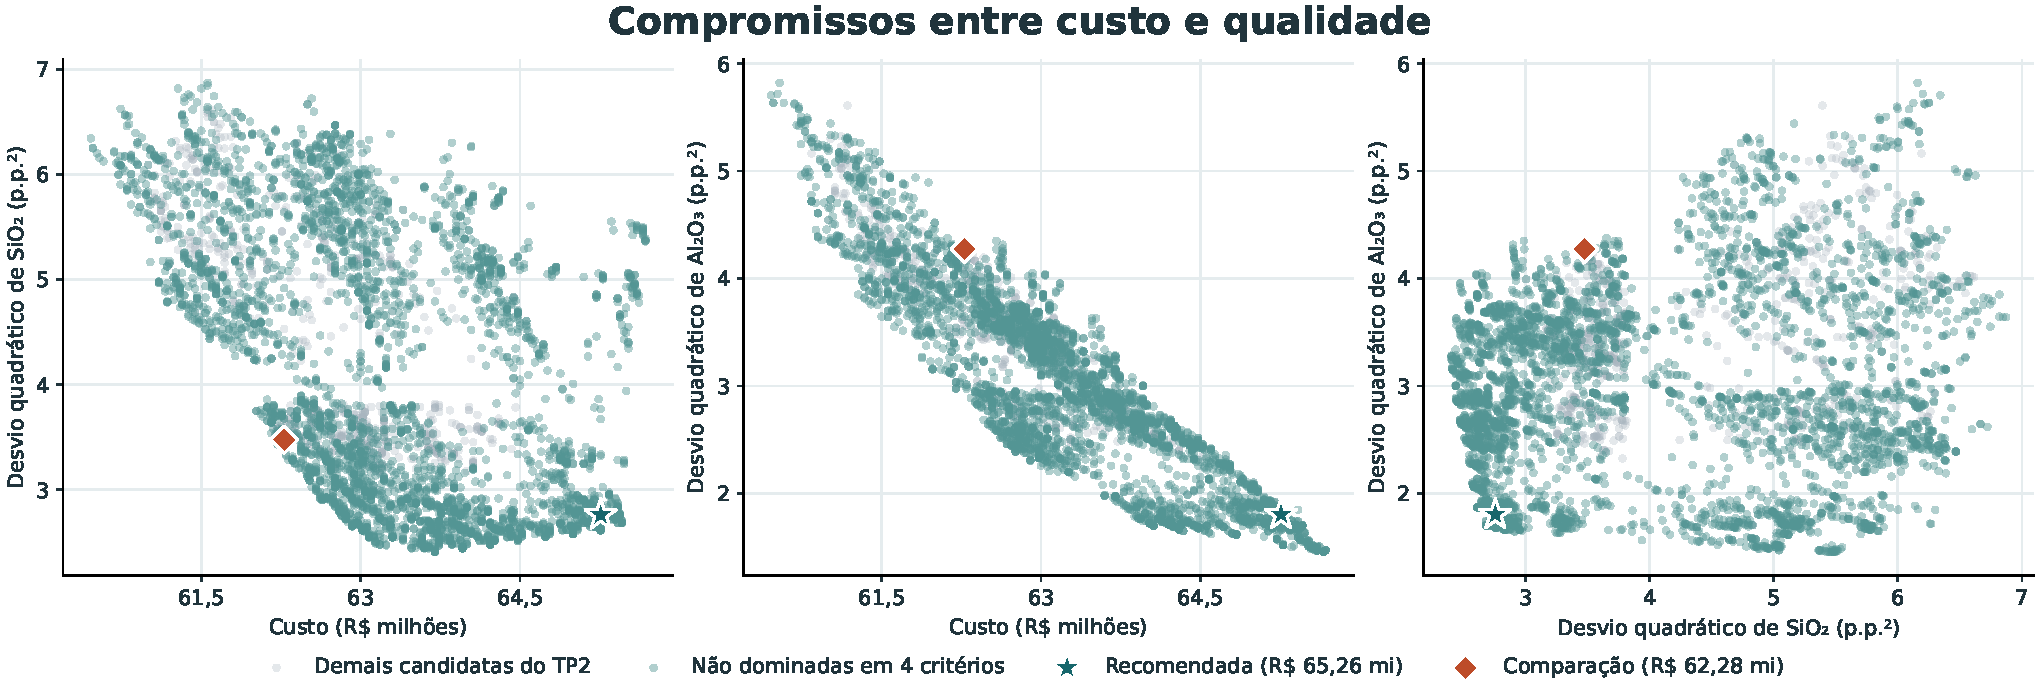
\includegraphics[width=\linewidth,height=8.11cm,keepaspectratio]{entrega_3/results_tp3_oficial/figuras/projecoes_objetivos.pdf}
\caption{Projeções custo \(\times\) sílica, custo \(\times\) alumina e sílica \(\times\) alumina. A estrela indica A01. O losango indica A02, vencedora do PROMETHEE II com 40\% de peso para custo.}
\end{figure}

As projeções mostram o compromisso com o custo. A opção de R\$ 62,28 milhões está à esquerda da recomendada nos painéis com custo, porém apresenta desvios químicos maiores. A classificação como não dominada usa os quatro critérios em conjunto. Os painéis projetam apenas os três objetivos da otimização e são utilizados para interpretar a escolha.

A recomendação de A01 é condicionada aos parâmetros do cenário-base. Se a operação estabelecer um teto de custo ou adotar um peso maior para economia, os resultados de sensibilidade oferecem alternativas a reavaliar. A preferência relativa também depende dos limiares considerados para distinguir diferenças pequenas e grandes.

\clearpage

\subsection{Composição e qualidade das pilhas recomendadas}

\begin{figure}[H]
\centering
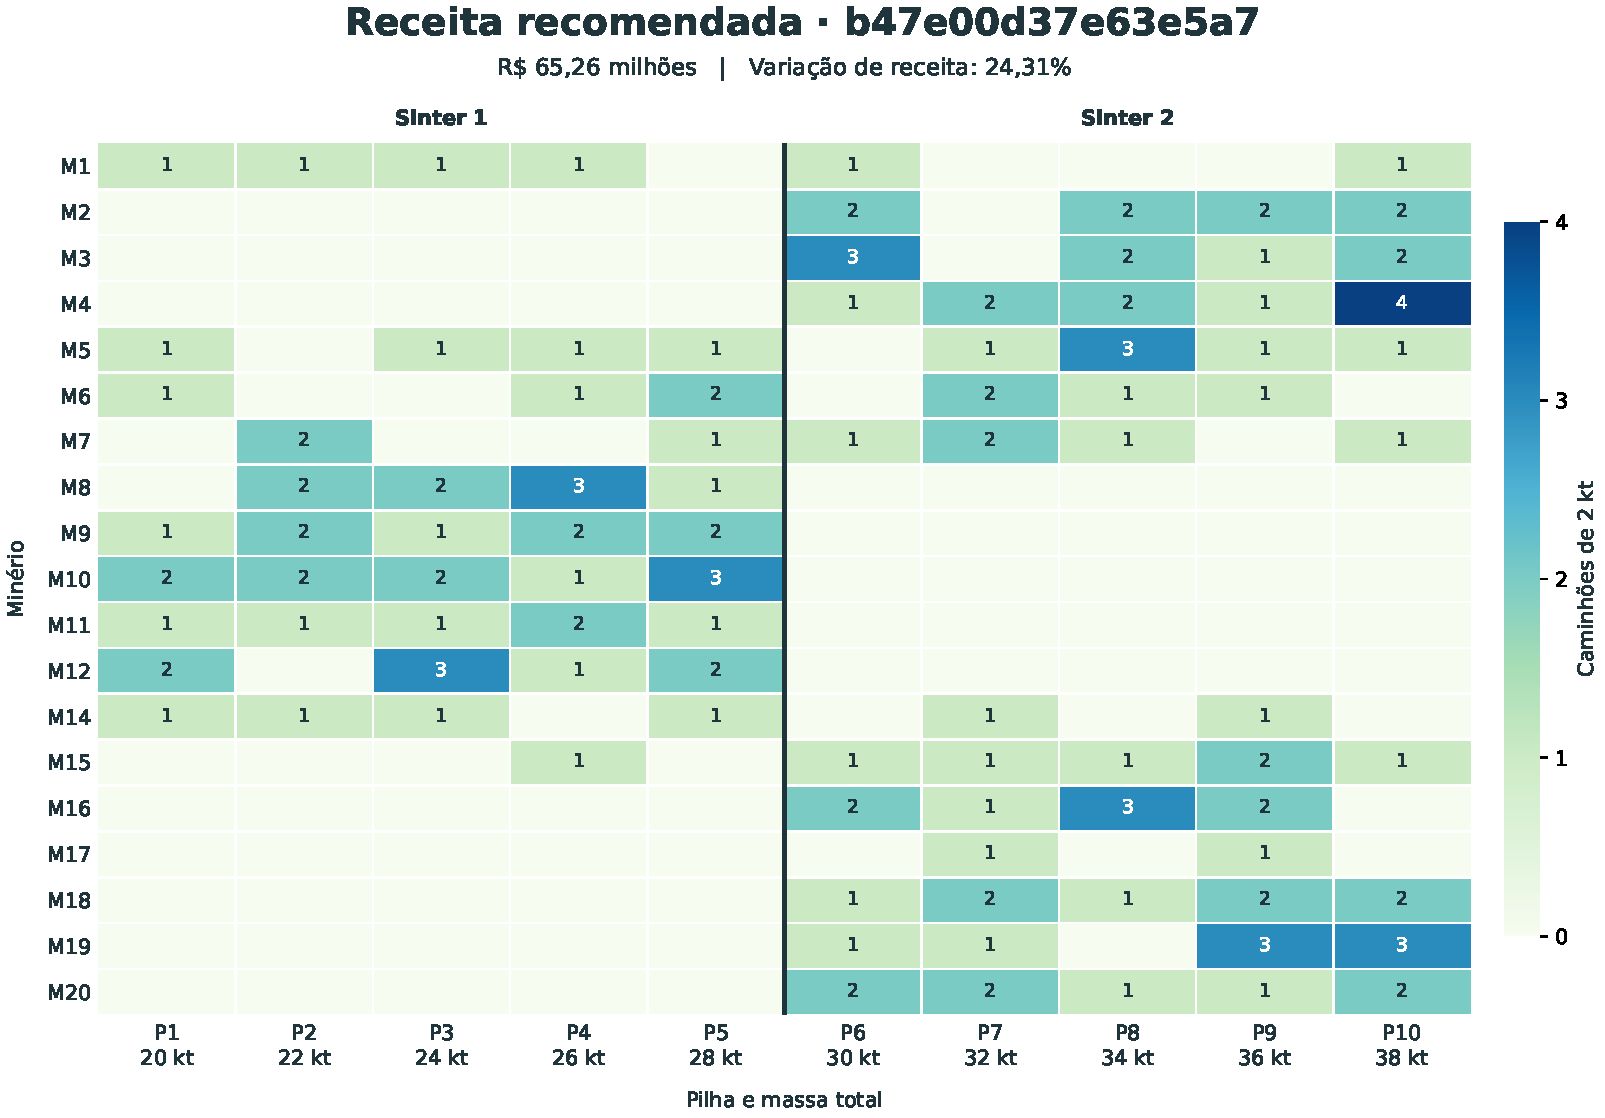
\includegraphics[width=\linewidth,height=10.05cm,keepaspectratio]{entrega_3/results_tp3_oficial/figuras/composicao_pilhas.pdf}
\caption{Quantidade de caminhões por minério e por pilha em A01. Cada caminhão corresponde a 2 kt. As células sem número correspondem a quantidade zero.}
\end{figure}

\begin{table}[H]
\centering
\small
\caption{Massa e teores recalculados para a composição recomendada.}
\begin{tabular}{@{}p{0.102\linewidth}p{0.102\linewidth}p{0.162\linewidth}p{0.162\linewidth}p{0.162\linewidth}p{0.162\linewidth}@{}}
\toprule
Pilha & Sinter & Massa (kt) & FeT (\%) & SiO\textsubscript{2} (\%) & Al\textsubscript{2}O\textsubscript{3} (\%) \\
\midrule
P1 & 1 & 20 & 60,400 & 5,930 & 1,530 \\
P2 & 1 & 22 & 61,091 & 6,009 & 1,545 \\
P3 & 1 & 24 & 60,250 & 6,000 & 1,558 \\
P4 & 1 & 26 & 61,308 & 6,023 & 1,608 \\
P5 & 1 & 28 & 60,214 & 6,071 & 1,607 \\
P6 & 2 & 30 & 60,667 & 6,027 & 1,947 \\
P7 & 2 & 32 & 59,625 & 6,025 & 2,038 \\
P8 & 2 & 34 & 60,529 & 6,106 & 1,906 \\
P9 & 2 & 36 & 59,333 & 6,094 & 2,056 \\
P10 & 2 & 38 & 60,000 & 6,158 & 2,068 \\
\bottomrule
\end{tabular}
\end{table}

As massas correspondem às dez metas da instância, e os teores de SiO\textsubscript{2} e Al\textsubscript{2}O\textsubscript{3} estão dentro dos limites dos respectivos equipamentos. Os desvios quadráticos medem a distância em relação aos alvos, mesmo quando o teor atende aos limites.

\clearpage

\subsection{Aplicação Streamlit}

A aplicação lê a mesma base de alternativas, rankings e cenários utilizada no relatório. A tela de alternativas permite selecionar a projeção, filtrar a fronteira em quatro critérios e comparar composições. A tela de rankings expõe a preferência de cada método e a sensibilidade. A tela de composição recupera a receita por pilha e os teores calculados com o modelo da instância.

\begin{figure}[H]
\centering
\IfFileExists{entrega_3/results_tp3_oficial/figuras/streamlit_alternativas.png}{%
  \includegraphics[width=\linewidth,height=4cm,keepaspectratio]{entrega_3/results_tp3_oficial/figuras/streamlit_alternativas.png}%
}{%
  \fbox{\parbox[c][4cm][c]{0.94\linewidth}{\centering Inserir captura da tela Alternativas, com a projeção e as composições destacadas.}}%
}
\caption{Exploração das alternativas e da fronteira no Streamlit.}
\end{figure}

\begin{figure}[H]
\centering
\IfFileExists{entrega_3/results_tp3_oficial/figuras/streamlit_rankings.png}{%
  \includegraphics[width=\linewidth,height=4cm,keepaspectratio]{entrega_3/results_tp3_oficial/figuras/streamlit_rankings.png}%
}{%
  \fbox{\parbox[c][4cm][c]{0.94\linewidth}{\centering Inserir captura da tela Rankings, com um cenário de sensibilidade selecionado.}}%
}
\caption{Comparação dos métodos e análise de sensibilidade no Streamlit.}
\end{figure}

\begin{figure}[H]
\centering
\IfFileExists{entrega_3/results_tp3_oficial/figuras/streamlit_composicao.png}{%
  \includegraphics[width=\linewidth,height=4cm,keepaspectratio]{entrega_3/results_tp3_oficial/figuras/streamlit_composicao.png}%
}{%
  \fbox{\parbox[c][4cm][c]{0.94\linewidth}{\centering Inserir captura da tela Composição, com a receita recomendada e os teores.}}%
}
\caption{Composição e qualidade das pilhas no Streamlit.}
\end{figure}

\clearpage

\section{Conclusão geral}

O estudo integrou três níveis de análise. A otimização mono-objetivo identificou referências individuais, a etapa multiobjetivo expôs compromissos entre os objetivos originais e a tomada de decisão acrescentou a uniformidade das receitas ao processo de escolha. As composições da campanha oficial permitiram comparar os métodos sobre a mesma matriz de decisão.

A01 foi selecionada por AHP e PROMETHEE II sob pesos equilibrados. A composição reúne o menor valor observado de variação de receita e desvios químicos próximos aos extremos individuais da campanha multiobjetivo. Seu custo de R\$ 65,26 milhões representa um acréscimo de R\$ 4,80 milhões sobre a alternativa de menor custo do arquivo oficial. A análise de sensibilidade quantifica como essa escolha responde a outras prioridades, especialmente quando o custo ou os limiares do PROMETHEE II são alterados.

A recomendação depende do conjunto de composições encontrado pelo GVNS, da instância e das preferências adotadas. Antes de aplicar a solução em outro período operacional, é necessário verificar as disponibilidades, as condições logísticas e os parâmetros de decisão correspondentes.

\subsection{Reprodução dos resultados}

Na raiz de entrega\_3, execute python -m src.main --entrada ../results/tp2/pareto --saida results\_tp3\_oficial. A execução consolida as alternativas e gera os rankings e a sensibilidade. Em seguida, execute python -m src.usecases.usecase\_figuras results\_tp3\_oficial para reproduzir as figuras. A aplicação é iniciada com python -m streamlit run app.py, após instalar as dependências do arquivo requirements.txt.

\section*{Referências}
\addcontentsline{toc}{section}{Referências}

SAATY, T. L. Decision making with the analytic hierarchy process. International Journal of Services Sciences, v. 1, n. 1, p. 83–98, 2008. DOI 10.1504/IJSSCI.2008.017590.

BRANS, J. P., VINCKE, P. e MARESCHAL, B. How to select and how to rank projects: The PROMETHEE method. European Journal of Operational Research, v. 24, n. 2, p. 228–238, 1986. DOI 10.1016/0377-2217(86)90044-5.

UFMG. Case UFMG 2026/2: Disciplina Teoria da Decisão. Otimização do custo e qualidade de pilhas de minério. Enunciado fornecido à turma, 2026.



\end{document}
